\section*{Response to Reviews}

\textbf{Submission:} EPDS-D-20-00186 \\
\textbf{Manuscript:} 
Allotaxonometry and rank-turbulence divergence: A universal instrument for comparing complex systems
\textbf{Authors:} Dodds et al.

\begin{editorcomment}[Assessment from the Associate Editor:]
  The authors propose a very interesting method. We're sorry this review
  took a long time, but eventually we were able to secure three highly
  competent Reviewers. Reviewer 1 presents a few major reviewer comments
  and recommended a major revision. Upon closer inspection, however,
  those reviewer comments are mostly interpretational, but addressing
  them will make the manuscript more readily accessible to a broader
  readership. The reviewer comments of Reviewer 1 are in line with the
  reviewer comments from Reviewer 2, who also suggests the authors make a
  few minor clarifications. Reviewer 3 raises no criticism. Taken
  together, all reviews are very positive and only minor clarifications
  are requested.
\end{editorcomment}

\subsection*{Overall remarks concerning our response to reviewers:}

\begin{enumerate}
\item 
  We deeply apologize for the delay in our response. The lead author
  has had a series of unfortunate maladies over a full year. This
  paper represents an enormous effort, and our response
  has required sustained time to
  engage with fully.
\item 
  We greatly thank the editor for their efforts and their overall positive evaluation.
\item 
  We greatly appreciate the helpful comments from their reviewers,
  and for their positive feedback.
  Their input has led to a number of substantive improvements.
\item 
  We have taken substantive time to revise the manuscript
  to properly address all concerns put forward by the reviewers, with individual responses below.
\item 
  For ease of reading, we have framed the comments from the reviewers in light blue boxes.
  We also show relevant edited excerpts from the updated manuscript in light gray boxes.
\item
  We have expanded our description of the allotaxonographs in Figs.~1 and 2.
  We have added overlaid dashed boundaries with labels to their many parts
  (10 parts for Fig.~1, and 6 parts for Fig.~2).
  We have extracted these (small) labeled graphical elements
  and then incorporated them in the text
  to better facilitate our explanation.
  We hope that this new structure will
  be acceptable for EPJ Data Science.
\item 
  We have also generally improved the manuscript with some minor edits throughout.
\item
  We note that our script for creating allotaxonographs also accommodates
  Probability Turbulence Divergence (PTD, described in a separate paper)
  and
  entropy-based divergences,
  e.g., Jenson-Shannon divergence (JSD) and a natural generalization.
\item
  We have added three more example allotaxonographs in response to reviewer's comments.
\item
  We have shared more code and data through
  the paper's Gitlab repository, and will aim to continue to build there.
  We intend that the paper's figures should all be rebuildable from scratch.
\item
  We have replaced Flipbook 3 which was a series of bare allotaxonographs
  for Twitter, rather than an intended series of allotaxonometric graphs.
\item
  We have also adjusted some terminology for clarity,
  and to remove unneeded attributions to individual scientists.
  For example, we have largely replaced ``Zipf distributions'' with
  the more
  plainspoken ``size rankings'', ``size-rank distributions'', and ``rankings''.
  (We still cite Zipf appropriately.)
\end{enumerate}

Overall, and while we have expended considerable time and effort
to respond fully and faithfully to the reviewers,
we have introduced no major changes in the manuscript.
As the editor indicated, we have found that only clarification
has been requested.

We note that that we received no comments about the mathematical
construction of rank-turbulence divergence, the core invention of
the paper.
As we have sought to demonstrate with our paper,
we have extensively demonstrated how allotaxonographs and RTD perform
for a range of disparate systems.
The core instrument remains the same as do all original figures,
except for Fig.~10 (was Fig.~7) which now includes more information.

We hope that our revised manuscript is suitable for publication in
EPJ Data Science.

\reviewerheader{1}

\begin{reviewercomment}
  Reviewer \#1: Thank you for the opportunity to
  review this paper. It proposes new methods to compare either
  multiple systems or a single system over time, including graphs and
  a measure of divergence. The proposed methods are demonstrated on a
  variety of data examples.

  Major Reviewer comments:

  Can we use the rank-rank histogram to detect differences in the number
  of component types between the two systems? For example, can we use
  the histogram to figure out whether there are more species in 1985
  vs. 2015 in Figure 3?
\end{reviewercomment}

As is, we do not make the total number of types explicit in the
rank-rank histograms. We have intended that our instrument will
work on bare rankings.

To further help make clear that rank-divergence works purely on rankings we have adjusted
a paragraph from the introduction to read:
\begin{excerpt}
  We will consider systems where
  each component type $\elementsymbol$ has at
  least one measurable---and hence rankable---``size'' $\sizesymbol_{\elementsymbol}$.
  We make clear that we may have no knowledge of these component sizes---we may only have rankings (e.g., book rankings provided by a seller,
  but with numbers of sales withheld).
  Our core instrument functions only on rankings,
  incorporating size data (if available) for minor diagnostics.
\end{excerpt}

That said, and as we note below, various absolute numbers
are returned within the Matlab environment when an allotaxonograph
is generated (and can be computed separately).

We provide three points.

1.
In general, our rank-rank histograms will strongly visually indicate if two
systems are imbalanced in their respective number of distinct types
(on this topic, see also our response to Question 5 from Reviewer 2).

For example, in Figs. 4 and 5, the allotaxonographs for baby girl and boy names
show a distinct line separated from the main histogram only on the 2018 (right hand) side.
Names that fall along this separated line are names that
appear in only 2018 (`2018-exclusive types').
So without the exact numbers of types, a user (with some familiarity)
will immediately see that there are more types
of baby names in 2018.

By contrast, the allotaxonograph for Twitter in Fig. 1 shows a fairly balanced number of types.
On both sides, we see two similarly separated lines from the main histogram, corresponding to 1-grams
that appear 0 times in the comparison corpus
(bottommost outer separated line) or 1 time (inner separated line).

2.
The script for generating allotaxonographs (figallotaxonometer9000.m in Matlab provided in the paper's Gitlab repository)
returns some diagnostics
including a set of absolute numbers (this output can be ignored).

Here's an example of part of the output,
using the 1968--2018 baby girl name comparison from Fig. 4,
and with comments added:
\begin{lstlisting}[language=Matlab]
  details = 
  struct with fields:

  Nunion: 22758    %% # of types in union of both systems
  Nshared: 3552     %% # of types in intersection of both systems
  N1: 8195     %% # of types in system 1 (baby girl names, 1968)
  N2: 18115    %% # of types in system 2 (baby girl names, 1968)
  N1exclusive: 4643     %% # of exclusive types in system 1
  N2exclusive: 14563    %% # of exclusive types in system 2
  totalcounts1: 1640302  %% Total # of girls in system 1 (token count)
  totalcounts2: 1696917  %% Total # of girls in system 2 (token count)
\end{lstlisting}

3.
(Note: Some form of the text below now appears in the manuscript.
See our answer to reviewer 1's third comment below.)

The balances at the bottom right of each allotaxonograph
(now labeled 1G in Fig. 1) present various
\textit{relative} comparisons derived from absolute numbers of types,
and if available, `sizes' of those types.
Size is often a form of counting (words, baby names) but could
be anything and may not be normalizable (e.g., market cap for corporations).

Again for baby girl names in Fig. 4, here's the extracted display of balances:
\begin{center}
  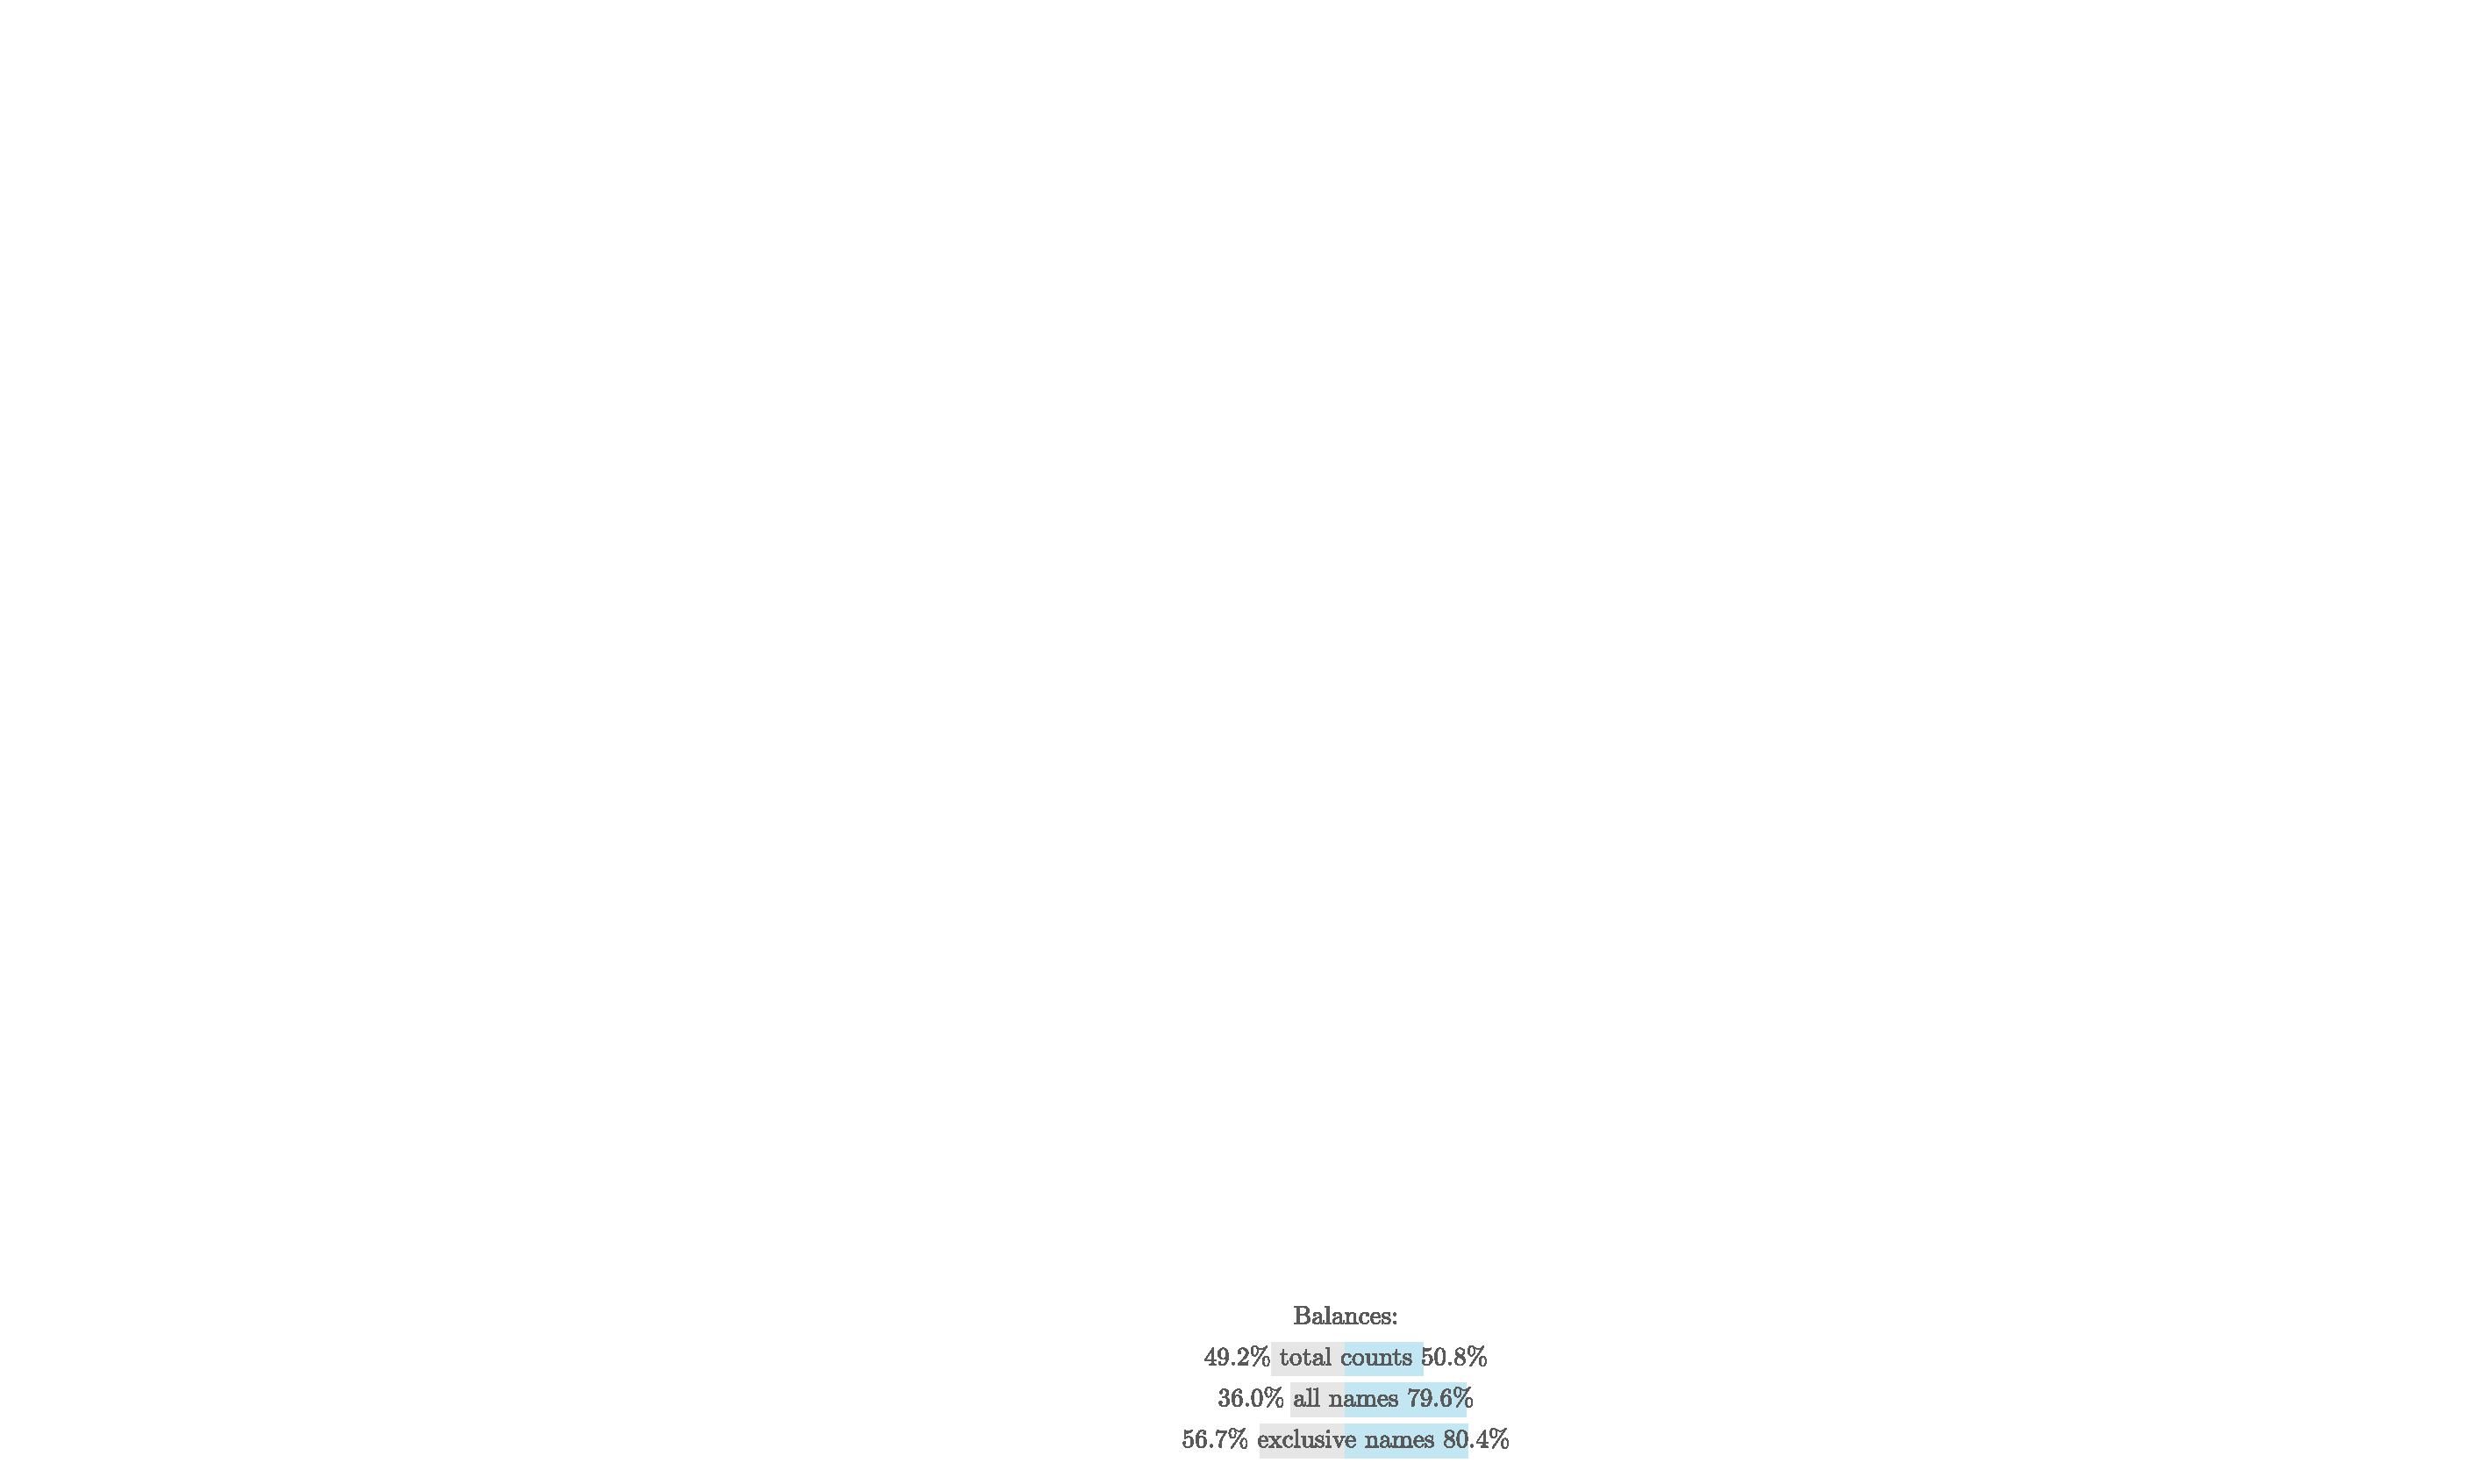
\includegraphics[width=0.3\textwidth]{figallotax-baby-girl-name-balances.pdf}
\end{center}

Each allotaxonograph will display two or three bars.
Per the reviewer's interest,
comparisons for the numbers of types in each system
are recorded in the bottom two bars,
and the top one, described below, is rendered optionally.

Counts of names (and more generally, sizes of types)
are not incorporated in the two bottom bars.

The second balance from the bottom shows the fraction of types in each system
as a percentage of the union of types from both systems.
For baby girl names, the computation is:
\begin{lstlisting}
  >> details.N1 / details.Nunion * 100 
  8195 / 22758 * 100
  ans =
  36.0093
  >> details.N2 / details* 100.Nunion * 100 
  18115 / 22758 * 100
  ans =
  79.5984
\end{lstlisting}
These numbers correspond to the middle of the balances: 36.0\% versus 79.6\%.

The bottom balance shows that given each side's set of types,
what percentage appears only on that side.
The computation is:
\begin{lstlisting}
  >>     details.N1exclusive / details.N1 * 100
  4643 / 8195 * 100
  ans =
  56.6565
  >>     details.N2exclusive / details.N2 * 100
  14563 / 18115 * 100
  ans =
  80.3919
\end{lstlisting}
And these numbers are shown in the bottom bar as 56.7\% and 80.4\%.

Lastly, a third bar will appear on top if we have measures of type size.
For baby names, we have counts and the computation is:
\begin{lstlisting}
  >> sumtc = details.totalcounts1 + details.totalcounts2  
  sumtc =
  3337219
  >> details.totalcounts1 / sumtc * 100                  
  1640302 / 3337219 * 100
  ans =
  49.1518
  >> details.totalcounts2 / sumtc * 100
  1696917 / 3337219 * 100
  ans =
  50.8482
\end{lstlisting}
The topmost of the three bars shows the relative balances for the two years:
49.2\% versus 50.8\%.

What the top balance bar shows is that the number of baby girls registered with social security has
increased only very slightly from 1968 to 2018.
The expansion of the `lexicon' of baby names is thus a strong one
and not an artifact of increases in sheer numbers.
We discuss this further in the manuscript.

We have added the following paragraph to the baby names secton:
\begin{excerpt}
  We emphasize that the balance indicators are for baby names
  appearing at least fives times. For our present work, and in
  attempting to maintain uniformity across allotaxonographs, we do not
  attempt to adjust for names appearing less than 5 times, though this
  would be possible for the topmost balance for total counts given we
  have that information separately. Clearly the balance values would
  shift if we had complete data sets for baby names; estimating errors
  for these estimates would be meaningful future work.
\end{excerpt}

%% For example, for baby girl names appearing at least 5 times in a year in the US,
%% there were 1,640,302 recorded in 1968 and 1,696,917 in 2018 (appearing means being
%% registered with Social Security).
%% 
%% Strong separation in the histogram for names that only appear in 2018 relative to 1968.
%% 
%% This means that we do 
%% 
%% In fact, there is only one optional 
%% 
%% This information is an figure-building code 
%% 
%% The top bar is optional and will only be present if a measure of ``size'' of each type is provided
%% along with the ranks.

%% \done{Point to balances}

%% \done{Add some text to paper about this.}

%% In future iterations, we could add the number of tokens
%% (if counts are the measure), number of types,
%% and number of exclusive types to the inset showing balances.
%% 
%% Add to discussion at end.
%% 
%% We note that the baby name allotaxonographs compare only ranked types.
%% 
%% The balance 
%% 
%% omitting the tail of any names that appeared less than 5 times in a year.
%% We do however have the total number of names for each year.

%% Thus, the three balances reflect the ranked names only

%% \done{Can see the imbalance from the histogram}

%% \todo{The numbers can be reported in text accompanying figures}



\begin{reviewercomment}
  Also, can we use the graph to gauge the difference in size
  between the component type of rank r in System 1 and
  the component type of System 2 of the same rank?
\end{reviewercomment}

As per our response to the question above,
for RTD, we wanted to build a tool that only works with ranked data.
While in practice, we will have systems where type `sizes' are known, the intent here
was to build a fully ranked-based instrument in the spirit of well established
rank-based statistical methods (e.g., the Spearman coefficient).

We add two points:

1. The main allotaxonometer script can produce allotaxonographs that
compare by only type size. These outputs will show only an allotaxonograph
with an annotated histogram and no overlaying measure of difference.

2. In our second paper on allotaxonometry, we introduce and explore
probability-turbulence divergence (PTD),
where we make size (as measured by probability or rate) explicit.
We note that the allotaxonometer code does include the ability to
compare systems where we have sizes that are not counts or
probabilities or cannot be interpreted as relative fractions in some
way (e.g., heights of buildings).
We construct PTD with a tunable parameter $0 \le \alpha < \infty$
in a similar fashion to RTD.
We show that PTD has different
limiting behaviors from RTD,
and that it matches up with a collection of existence
difference measures
including
$L^{(p)}$ norms,
the S{\o}rensen-Dice coefficient
(the $F_1$ statistic),
and 
the Hellinger distance.

We add that we prefer PTD over the commonly used Jenson-Shannon divergence (JSD),
which we have a separate article about, not yet on the arXiv.
JSD creates a mixture of two systems which does not exist
(half Moby Dick, half Pride and Prejudice for example).
PTD works as a true difference and is what one would want
in constructing a form of ``type calculus'' (``lexical calculus'' for text corpora).
Our allotaxonograph script nevertheless will produce JSD comparison plots,
along with a particular generalized entropy divergence.

The PTD manuscript can be found here: \url{https://arxiv.org/abs/2008.13078}

We note that we had mentioned type calculus and lexical calculus in the conclusion:
\begin{excerpt}
  Allotaxonometry may be viewed as part of a larger analytic
  framework of ``lexical calculus'' and, more generally, ``type calculus.''
\end{excerpt}
We have now added ``type calculus'' to the abstract.

\begin{reviewercomment}
  How do we interpret the percentages in the ``Balances'' section at the bottom of Figure 1? Are these percentages unrelated to your alpha tuning parameter? 
\end{reviewercomment}


For an overview of the Balance percentages,
we point back to our response to Reviewer 1's question 1 above.

We add here that the balances are independent of alpha, and indicate relative percentages
of type sizes (e.g., word counts), types, and exclusive types.

As we mention in the overview for our reply,
we have outlined 10 distinct cutouts of the allotaxonograph
in Fig.~1 to help with our discussion.
We have taken these cutouts and added them to
the text to, we hope, greatly help the reader with being
able to comprehend the instrument.

We describe balances in Sec IIB: ``Rank-Rank Histograms for Basic Allotaxonomy''.
The cutout for Fig.~1 for balances is Fig.~1G and can be found looking through
the subsections of Sec IIB.

We reproduce the relevant text here:

\begin{center}
  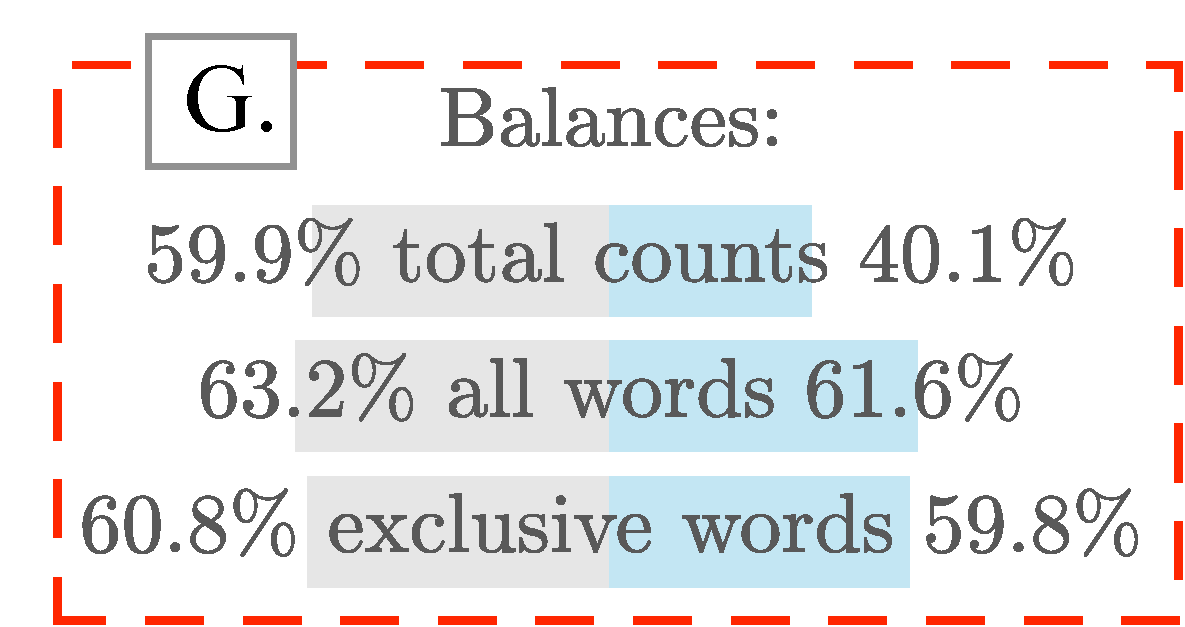
\includegraphics[width=0.4\columnwidth]{allotaxonograph_balances2_flattened-crop.pdf}
\end{center}
\begin{excerpt}
  \textbf{Fig.~1G}:
  For all allotaxonographs, we show balances at the bottom right
  of the rank-rank histogram.
  Two kinds of exclusive type comparisons for the numbers of types in each system
  are recorded in the bottom two bars,
  while the top bar conveys information about type sizes.
  The top bar is rendered only when sizes are known
  (this is the only part of the allotaxonographs that is not
  determined purely from type rankings).
  In the present paper, we work from datasets with known type sizes,
  and all allotaxonographs will have all three bars.
  All balances show normalized quantities rather than absolute numbers

  As we will see, these three balances can vary greatly across system comparisons.

  The top balance bar shows the relative balance of the two systems' sizes, if known.
  For our Twitter example, 
  this top bar shows the breakdown of total counts of 1-grams (type size)
  between the two dates at 59.9\% and 40.1\%.
  We thus see that the election generated considerably more tweets than Charlottesville.

  The middle balance bar shows the fraction of types in each system
  as a percentage of the union of types from both systems.
  For Twitter, we have that of all words in the combined lexicon for the two days combined,
  just over 60\% appear on each of the two days (63.2\% and 61.6\%).

  The bottom balance bar shows that given a system's set of types,
  what percentage of those types appear only in that system.
  For the Twitter example, we take the  separate lexicons for each day,
  and find that around 60\% of words are exclusive for both days,
  further giving a sense of strong turnover (60.8\% and 59.8\%).

  We add that the script for generating allotaxonographs
  (figallotaxonometer9000.m in Matlab provided in the paper's Gitlab repository)
  returns some diagnostics
  including the underlying numbers used to compute the above balances.
\end{excerpt}




%% \noway{we have also expanded the balance section to included absolute numbers}.

\begin{reviewercomment}
  The paper states that the standard methods lack transparency and flexibility.
  It may be helpful to apply some standard methods in one of your case studies to demonstrate the differences from your method.
\end{reviewercomment}

In preparing this manuscript,
we had separated out work where we compare methods (e.g., JSD vs RTD vs PTD),
but we had left residual guidance in the abstract.
This work is still being written up (as mentioned above).

We have removed two sentences from the abstract that misleadingly pointed
in the direction of other measures being deficient.
We have also removed any similar statements in the main text.

\begin{reviewercomment}
  How sensitive is your method to small perturbations? For example,
  if you fixed the errors in the Berkshire Hathaway and DowDuPont market
  caps in the last case study, how much do the divergence and histogram change?
\end{reviewercomment}

In general, using ranks will give a more robust instrument,
and is a key part of our overall motivation.

From the paper:
\begin{excerpt}
  Fourth, rank orderings
  potentially allow for powerful and robust non-parametric statistical measures
  such as Spearman's rank correlation coefficient.
  All told,
  while in moving from sizes to rankings
  we may
  trade information for some simplification,
  we still preserve a great deal of meaningful structure.
\end{excerpt}

We understand the reviewer's point, however,
that we could perform a deep analysis of sensitivity.
In this foundational paper, we have explored the effects of truncation only,
and reserve further work for later (by us, and, hopefully, others as well).
We believed (and continue to believe) that
the few small clear errors in the market cap database were worth
leaving in to show how outlier kinds of errors are easily observed
with allotaxonographs.

The above said, we corrected the Berkshire Hathaway and DowDuPont data
and recomputed $\rtd{1/3}$, finding it be unchanged to three significant figures
at 0.411.
The adjusted allotaxonograph (which we have added to the paper, and is included in our response below)
now make Berkshire Hathaway clearly ascendent
on the right side, as it was ranked 5th overall by market cap at the end of 2018.

Per the above, we have also added the following to the manuscript:

\begin{excerpt}
  The dataset for market caps does
  have some missing and erroneous data.
  DowDuPont's market cap for the last quarter of 2018 is absent
  and is consequently shown to have plummeted from
  a rank of
  $\sizerank$=91 in 2007
  to equal-to-last in 2018
  Berkshire Hathaway's
  market cap is clearly misrecorded
  for the last three
  quarters of the dataset
  (apparently dropping from
  \$528.33B
  to
  \$0.34B at the end of 2018).

  We take the opportunity to perform a small test of the sensitivity of rank-turbulence divergence
  by correcting the data for these two companies.
  For DowDuPont, with further sourcing, we find
  the year-end 2007 and 2018 market caps were reported as
  \$37.06B
  and
  \$121.34B,
  and for
  Berkshire Hathaway,
  \$149.56B
  and
  \$502.37B.
  Upon making these corrections, we first find again
  that $\rtd{1/3}$=0.411, unchanged to three decimal places.
  both.
  In the corrected allotaxonograph (Fig.~9),
  Berkshire Hathaway's location shifts to the right
  side of the histogram ($\sizerank$=38$\rightarrow$5)
  and is now listed as the 7th overall strongest contribution
  for $\rtd{1/3}$.
  DowDuPont no longer makes the top 40 of
  the list of contributions.
  While these two changes are dramatic,
  the remainder of the allotaxonograph
  remains essentially identical.

  Nevertheless, we have chosen to leave such errors in
  Fig.~8
  to help demonstrate the importance of using a rich,
  graphical allotaxonometric instrument.
  With a naive measurement of divergence, we would easily miss problematic data points.
  Evidently, and beyond our present paper's interests,
  for any further investigations,
  these two errors suggest that considerable effort should
  be made to further clean the market cap dataset
\end{excerpt}

\clearpage

For ease of comparison, we include both the
uncorrected and corrected market cap allotaxonographs below (Figs.~8 and 9)
and the corrected one below.

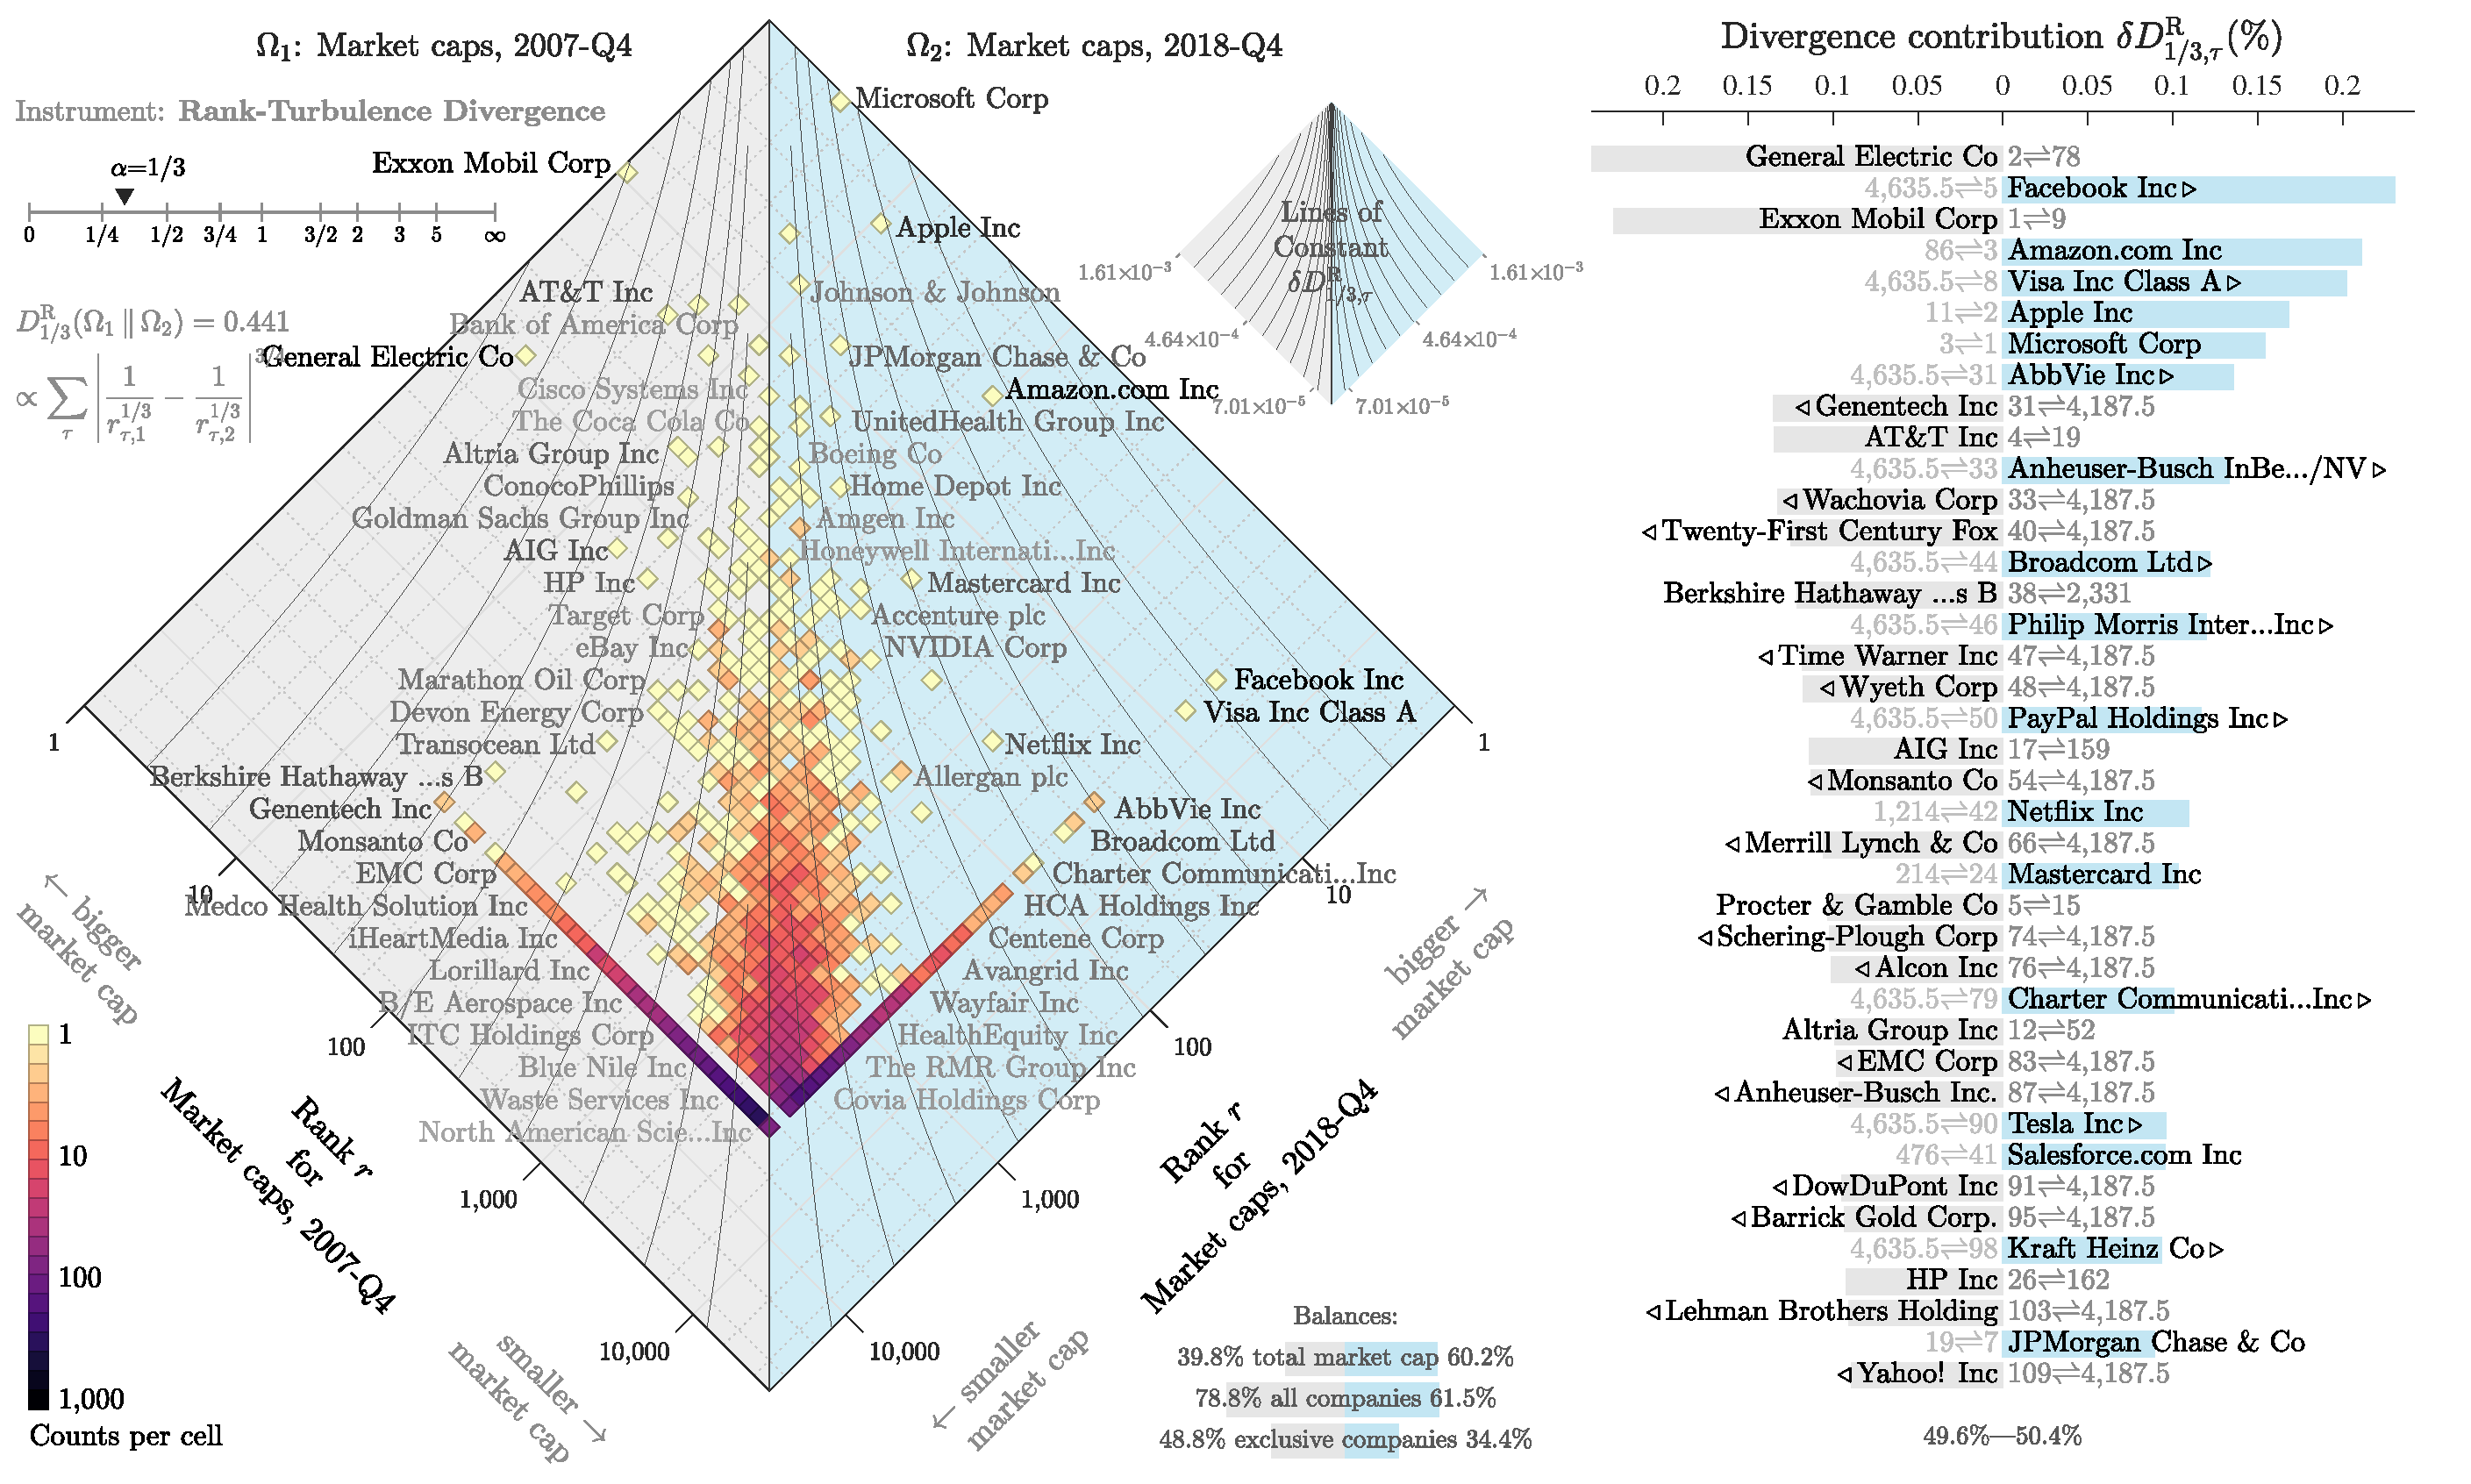
\includegraphics[width=\textwidth]{figallotaxonometer9000-siblis_alphasweep_05-2007-Q4_2018-Q4_marketcaps004_noname.pdf}

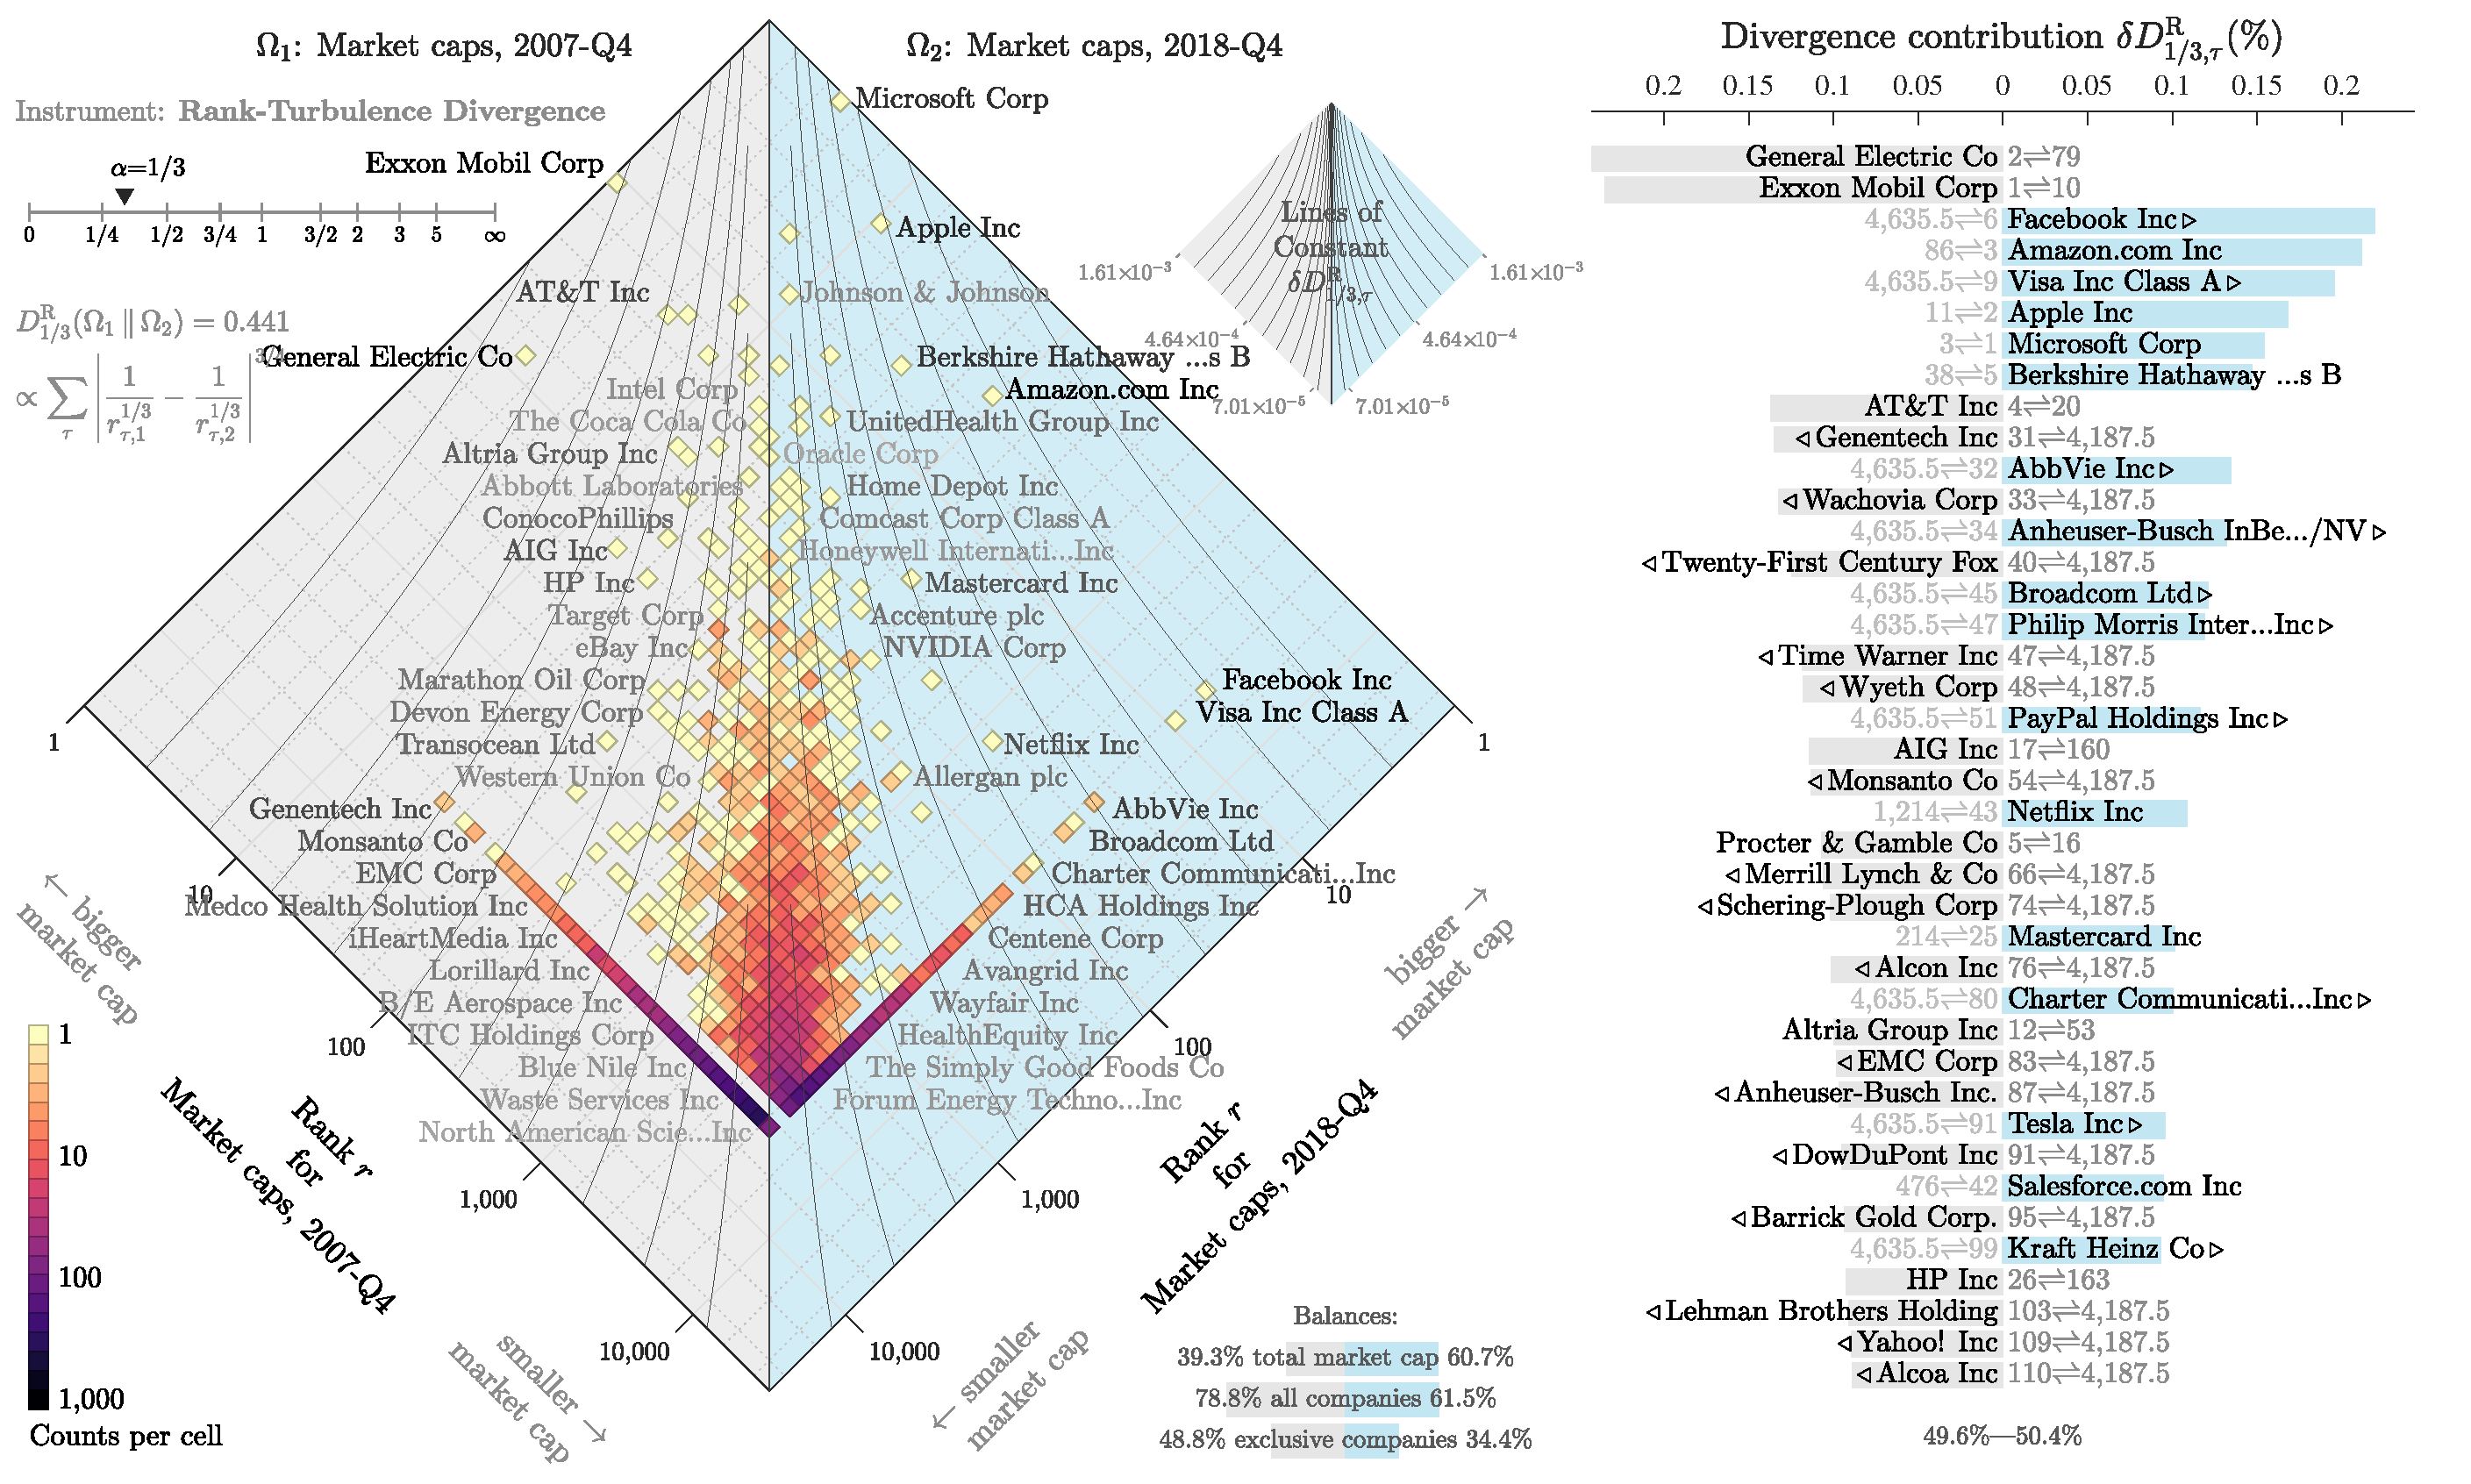
\includegraphics[width=\textwidth]{figallotaxonometer9000-siblis_alphasweep_06-2007-Q4_2018-Q4_marketcaps004_corrected_noname.pdf}

\clearpage

Caption for second figure:
\begin{excerpt}
  \textbf{Allotaxonometric comparison of publicly traded US companies
    in 2007 and 2018 by fourth quarter market capitalization
    with corrections for Berkshire Hathaway and DowDuPont Inc.}
  To be compared with Fig.~8.
  The 2018 market caps for both these companies were recorded incorrectly
  in the original data set.
  The revised allotaxonograph shows Berkshire Hathaway---which in fact rose to
  $\sizerank$=5 in 2018---now appears prominently
  on the right hand side of the histogram and the contribution list.
  DowDuPont Inc's corrected rank for 2018 means that it did not
  contribute as strongly, and now no longer appears in the top 40 contribution list.
  Overall, the allotaxonograph is largely identical to that
  of Fig.~\ref{fig:rankturbdiv.allotaxonometer9000-siblis_2007-Q4_2018-Q4_marketcaps004}.
  The rank-divergence is unchanged at $\rtd{1/3}=0.411$.
\end{excerpt}


\begin{reviewercomment}
  What is the computing time to calculate the divergence and generate
  the histograms in your four case studies?
\end{reviewercomment}

Generally, the calculations and graphics require a few seconds of
compute time.
In our experience, the only speed limitation arises
when loading massive datasets (e.g., Twitter).
Separate from our analyses, computational preparation of such large datasets
is where we see delays.
For the Twitter data, for example, enumerating $n$-grams for each day
(20GB of compressed text) can take many CPUs running continuously to
keep up with real time, with more than one million previously unseen
types encountered on a given day.

The computational bottleneck in producing the RTD
calculations is confined entirely to the counting of elements to
produce ranks.

\begin{reviewercomment}

  Minor Reviewer 1 comments:

  \bigskip

  The terms ``Zipf'' and ``1-gram'' should be defined.

\end{reviewercomment}


We have made the initial reference to Zipf more clear, connecting only to ``Zipf's law''.
We have also now defined Zipf distribution and $n$-grams in the manuscript. 
We have replaced ``Zipf ranking'' with ``size ranking'' throughout, as we do not need
to name this simple kind of ranking after an individual
(we of course cite Zipf and others where appropriate).

Added to the manuscript:
\begin{excerpt}
  Here, we will refer to such
  ``a component ranking by decreasing size'' as a ``size ranking''
  or, for brevity and given our paper's framing, simply a ``ranking''.
\end{excerpt}

In the main text, we have added this definition/clarification of $n$-grams when the term first appears:

\begin{excerpt}
  For Twitter, subsampling $n$-grams---phrases containing $n$ consecutive words and/or other text elements---allows for robust estimation of the rates of common $n$-grams but not rare ones.
\end{excerpt}

And in the caption of the Fig.~1:

\begin{excerpt}
  Words are extracted first as 1-grams (contiguous sets of non-whitespace characters)
  from tweets identified as English \ldots
\end{excerpt}


\begin{reviewercomment}
  In Paragraph 2 of Part B in the Introduction, it would be helpful to
  get a concrete example of a component type.
\end{reviewercomment}

We have added an explanatory paragraph at the start of section B in the introduction,
as well as pointed to this when we first mention size.

In ``Sec. I. Introduction A. Instruments that capture complexity'', we now have:
\begin{excerpt}
  But for complex phenomena made up of
  a great many types of components
  of greatly varying `size'
  (clarified below in Sec.~I B)---language, ecologies,
  stock markets---we
  must confront two major problems with our dashboards of simple instruments [2].
\end{excerpt}
We have put size in quotes to indicate it should be construed more generally, or at least,
that the reader will need to see our description.

Then in ``Sec. B. Size rankings, Zipf’s law, and rank turbulence'' (we have removed ``Zipf distributions'' from the title of this section), the section begins with:

\begin{excerpt}
  While the instrument we develop here will have broader application,
  its construction focuses on two regular features of complex systems:
  Heavy-tailed `size-rank distributions' (rather than laws),
  and
  what we will call `rank turbulence'---a phenomenon of system-system comparison.
  We describe and discuss these two common signatures of complex systems in turn.

  We will consider systems where
  each component type $\elementsymbol$ has at
  least one measurable---and hence rankable---`size' $\sizesymbol_{\elementsymbol}$.
  To help make clear what we mean by component types and component sizes,
  we list some examples in the realms of language, ecology, and stock markets.

  \begin{itemize}[leftmargin=70pt]
  \item[Example types:]
    `the', `love', and `spork'.
  \item[Type size:]
    Number of times a word appears in a book.
  \end{itemize}
  In ``Pride and Prejudice'', for example,
  the corresponding counts are
  %% 498, %% !
  4,058, %% the
  90, %% love
  and
  0. %% spork
  In linguistics, the component type and component size distinction is
  referred to as types and tokens [10],
  while more abstractly in semiotics, we have the signifier and the signified.

  \begin{itemize}[leftmargin=70pt]
  \item[Example type:]
    The species Ornithorhynchus anatinus, the platypus.\\
  \item[Type size:]
    The number of platypuses (`instances' of the species) living in Australia in the wild.\\
  \end{itemize}
  Given an ecology, species may be ranked by their population numbers.

  \begin{itemize}[leftmargin=70pt]
  \item[Example types:]
    The publicly traded companies of Apple and Microsoft.
  \item[Type size:]
    Market capitalization.
  \end{itemize}
  Apple and Microsoft may be viewed as components of the publicly-owned corporate world.
  The sizes of corporations may be broken down into many rankable dimensions
  such as annual revenue or number of employees worldwide.
  Market capitalization represents a kind of current collective belief
  in terms of money.

  The three examples above show some of the range of what size can mean, and why we
  cannot readily lift terminology out from one domain to apply to all.
  Size for a word in a corpus means the number of indistinguishable instances of that word
  (many identical entites---tokens);
  size for species means the number of `biological replications' of an individual type
  (many genetically similar entities of varying ages);
  and
  size for a corporation means a monetary value (one entity).

  %% grep here:
  %% ~/work/stories/2021-02ousiometer-books/data/2020-08gutenberg-jane-austen/narrativetimeseries
  %% grep ^the\$ pride_and_prejudice_narrativetimeseries.txt | wc

  Some further examples of component size
  are
  %% counts (e.g., of words in text corpora),
  rate (e.g., appearance of words in streaming text),
  physical dimensions (e.g., typical animal length or weight for a species),
  social popularity (e.g., number of plays of a song)
  scoring in sports by individual players,
  and so on.

  We make clear that we may have no knowledge of
  the underlying component sizes---we may only have rankings
  (e.g., book rankings provided by a seller,
  but with numbers of sales withheld).
  Our core instrument functions only on rankings,
  incorporating size data (if known) for minor diagnostics.
\end{excerpt}

\begin{reviewercomment}
  Define the notation $r_{\tau,1}$ and $r_{\tau,2}$ , which seems to be
  first used in Part B of Section II. I believe they are the ranks of
  component $\tau$ in Systems 1 and 2, but this should be clarified.
\end{reviewercomment}

The reviewer reads the notation correctly, even though, as the reviewer notes,
we did not formally provide a definition.

To correct this oversight, we have added the following sentence as
a standalone paragraph (now the third paragraph of Sec. II B):

\begin{excerpt}
In general, we will denote the rank of type
$\elementsymbol$
in system $\systema$
by
$\sizerank_{\elementsymbol,\indexaraw}$,
and
its rank
in system $\systemb$
by
$\sizerank_{\elementsymbol,\indexbraw}$.
\end{excerpt}


\begin{reviewercomment}
  In Figure 1, the caption has substantial overlap with the main
  text. Removing some of the overlap would help highlight the new
  information.
\end{reviewercomment}

It is our firm preference to make the captions reasonably complete
in themselves.
Readers may choose to work through the paper in different ways.

\begin{reviewercomment}
  In the first two paragraphs on page 6, some of the words that are
  described (such as ``Harambe'' and ``voted") do not seem to be in
  Figure 1.
\end{reviewercomment}

Many thanks for pointing this out---we appreciate the reviewer's
careful reading.

Generally speaking for rarer types, each run of the allotaxonometer
script may have different annotations automatically rendered.
There are a number of reasons, mainly if annotation spacing is changed,
or if a particular rank-rank pair is held by more than one type.
In the latter case, the annotated type will be randomly chosen,
and for some comparisons this means the rendered allotaxonometer will
always be different.
For example, for two days on Twitter in our data et,
the number of 1-grams that appear once on one day and not on the other
run into the millions.

We have adjusted the language describing
Fig.~1 to match words found at the edges of the histogram. `Gorilla'
appears in the figure, so we have been able to retain a description of Harambe for
context in the main text.

%% \done{double check that remade figure contains words referenced in the caption}

\begin{reviewercomment}
  Could you give some intuition of why you chose $\alpha = 0$ for the
  BCI example?
\end{reviewercomment}

We make the choice of $\alpha = 0$ by inspection.
In the appropriate supplementary PDF flipbook, the effect of tuning alpha can be observed.
Future work, which we discuss at the end of the paper, would seek to find
a method to determine an optimal alpha for specific comparisons.

A secondary aspect of the choice to use $\alpha = 0$ is simply to demonstrate
how such an allotaxonograph looks.
The BCI example, with its limited rank
turbulence and vertical shaping within the histogram, provides 
a good instance where $\alpha = 0$ is at least visually reasonable.
A choice of $\alpha = 0$
would make for a poor fit for the Twitter example (and for written texts in general).

We have revised and expanded the section reference by Reviewer 1.

\begin{excerpt}
  We numerically compare the 1985 and 2015 distributions by applying
  rank-turbulence divergence with $\alpha = 0$,
  finding $\rtdalphavarsystemsRank{0} = 0.077$.
  By inspection, we choose $\alpha=0$ here
  because of the match of the histogram
  with the verticality of the contour lines
  (we address optimal selection of $\alpha$ in our concluding remarks).
  The nature of the BCI example affords us an opportunity to
  demonstrate the limit of $\alpha=0$ for allotaxonometry,
  and is a secondary reason for including an example from ecology.

  In Flipbook \flipbooktrees, we show how the allotaxonometer
  performs with $\alpha$ varying away from 0 to $\infty$.
  The visual match on the contour lines continuously degrades.
\end{excerpt}

\begin{reviewercomment}
  Also, what is the $D_{0;\,\textnormal{rand}}^{\textnormal{R}}$ term
  mentioned in that example?
\end{reviewercomment}

We have now explained what we mean by a randomized version,
and explicitly connected this explanation to the notation.

The section (which directly continues on from the excerpt above)
now reads:
\begin{excerpt}
  The BCI example's histogram is far 
  from what we would expect of randomized systems
  (Fig.~1I).
  To see how RTD quantifies the difference between an observed system the randomized version,
  we construct a set of pairs of randomized systems,
  measuring rank-turbulence divergence for each.
  We do this by randomly permuting the species names within each system
  while leaving species counts fixed,
  thereby keeping the size-rank distributions the same.
  We can perform such a randomization for any system-system comparison
  (and we do so below again for baby names).

  We denote the average randomized divergence for two rankings 
  $\bigrank_{\indexaraw}$
  and
  $\bigrank_{\indexbraw}$
  as:
  \begin{gather}
    \rtdalphavarsystemsRankRand{\alpha}.
    \label{eq:rankturbdiv.randomizeddivergence}
  \end{gather}

  For the BCI example, we find that the score
  $\rtdalphavarsystemsRank{0} = 0.077$
  is well short of the randomized equivalent
  of
  $\rtdalphavarsystemsRankRand{0} = 0.376$
  (average of 100 randomizations; standard deviation $\sigma$=0.012).
\end{excerpt}

The quantity $\rtdalphavarsystemsRankRand{0}$
appears explicitly in the paper twice,
once in the BCI section (Sec. II C),
and once in the baby girl name section (Sec II D).


We have also made the first appearance of our general notation for RTD
a standalone equation (now Eq. 1).

\begin{excerpt}
  \begin{gather}
    \tag{1}
    \rtdalphasystemsOmega.
    \label{eq:rankturbdiv.rankturbdiv_defn}
  \end{gather}
\end{excerpt}

%% \done{Connect rand properly back to normalization and notation definition, or wherever}

\reviewerheader{2}

\begin{reviewercomment}
  It was my pleasure to review this article introducing a new
  framework to compare heavy-tailed ranked lists.  Specifically, the
  work motivates and derives a novel divergence measure for ranked
  lists, and then illustrates its usefulness across four examples
  including: Twitter word frequency, baby name popularity, species
  abundance, and firm sizes.

  The presentation is rich and clear, elucidating the central
  framework and offering wonderful insights into the motivating
  examples and applications.  The problem this article addresses is
  relevant to a broad range of data science applications.

  Therefore, I strongly recommend to publish the article in EPJ Data
  Science.
\end{reviewercomment}

We are delighted by Reviewer 2's very positive feedback.

\begin{reviewercomment}
  Reviewer comments: Even through the presentation is quite clear, it
  may benefit from an organization that extracts a few non-technical
  discussions from the rest of the text - i.e. a clearly identified
  general audience guide to allotaxonomy and the application of
  rank-turbulence.  This could support usage in fields outside of
  physics / data sciences.
\end{reviewercomment}

Thank you.

We will author a blog post and a Twitter thread to accompany
formal publication of the
manuscript that will advertise the utility of the instrument to other
disciplines.

We are also working on a Python and hopefully Julia version of the
allotaxonometer code (the original code was developed in Matlab) to
enable and encourage broader adoption.

We and others have also used allotaxonographs in a number of other
papers, and we now cite some of these in the manuscript's conclusion.

Our intent is that our foundational paper be thorough and detailed,
and will serve as a reference text, and we hope that the examples are illuminating
and inspirational.

\begin{reviewercomment}
  Relatedly, it would be helpful if the authors could elaborate on
  section IIE and the processes used to select different values of alpha
  for the different applications.  I'm imagining the framework being
  used by a non-expert who just keeps whatever default value of alpha is
  encoded instead of exploring the full range - or on the flip side,
  being overwhelmed with the many potential choices of alpha and not
  understanding what features of the histograms are being accentuated by
  the divergence in different limits. Can you distill a few guiding
  principles or questions to help motivate an appropriate selection?
\end{reviewercomment}

We have improved our discussion of the choice of $\alpha$ in the conclusion,
as well as given this discussion its own subsection (see excerpt below).

In this initial work, we justify the choice of alpha by looking at the shape of
rank-rank histogram as a guide.
The rank-rank histogram also immediately shows us when type (or lexical) turbulence is not
present (e.g., when the type rankings for the two systems are random shufflings of each other).

In short, our advice for readers is to use the visual help of the allotaxonographs.
In some of the supplementary PDF flipbooks, the effect of tuning alpha can be observed,
and readers can see how RTD behaves when the fit is good or bad.

In follow up work that has proved difficult, and which we discuss at the end of the paper, 
we  hope to identify a computational method to determine an optimal alpha for specific
comparisons.


\begin{excerpt}
  \subsection*{VI~C. Determination of $\alpha$}
  In our initial work, we have made the choice of the tuning parameter for
  rank-turbulence divergence, $\alpha$, a visually guided one.
  The user gains much from inspecting the rank-rank histogram alone,
  and, in our experience, is then readily able to choose an $\alpha$ for
  which the allotaxonometric contour lines best match the form of the histogram.
  A visually guided choice will be sufficient in cases of comparing two or a small
  number of systems.

  When rank turbulence presents as a scaling law---which is regularly the case
  for text corpora (e.g., Twitter, books)---we would want to be able to determine an optimal $\alpha$.
  While for generalized entropy approaches for single systems, the limit of
  linear scaling and Shannon's entropy demarcate the boundary
  between accentuating the common or the rare [7, 33, 53, 54], 
  we have found that for system comparisons, the optimal value of $\alpha$, if it exists,
  is dependent on the pair of systems being compared---there is no universal value.

  Generally speaking for text corpora, as two texts become more distinct,
  the optimal $\alpha$ increases.
  This is particularly clear for a corpus like
  Twitter, for example, where rank turbulence increases with the
  calendrical separation of two dates being studied.

  We have left open the
  possibility of an analytic
  connection between the rank-turbulence scaling described
  at the end of Sec. I B,
  and, to the extent that well-defined scaling is present,
  with an optimal $\alpha$ for rank-turbulence divergence.

  Even with an optimization method for determining $\alpha$, we urge readers to
  always look at the visuals provided by our allotaxonographs---the maps---for confirmation of fit.
\end{excerpt}

\begin{reviewercomment}
  The examples illustrating the effects of partial sampling were
  helpful, but it would be nice to see how the divergence measure
  itself changes with subsample size: does it converge or is it
  sensitive to the influx of different cross-ranks uncovered by larger
  subsample sizes?
\end{reviewercomment}

First, for each of the five main case studies,
we do in fact show the full allotaxonographs in the series of
Flipbooks S10, S11, S12, S13, and S14 in the
supplementary material.

From Sec IV. Guide to Flipbooks,
here is our description of these flipbooks:
\begin{excerpt}
  \textbf{Flipbook \flipbooktwittertrunc---Word use on Twitter, truncated:}
  Full series of allotaxonographs 
  corresponding to histograms of
  row 1 in Fig.~7 with $\alpha=1/3$.

  \smallskip
  \textbf{Flipbook \flipbooktreestrunc---Tree species abundance, truncated:}
  Full series of allotaxonographs 
  corresponding to histograms of
  row 2 in Fig.~7 with $\alpha=0$.

  \smallskip
  \textbf{Flipbook \flipbookgirlnamestrunc---Baby girl names, truncated:}
  Full series of allotaxonographs 
  corresponding to histograms of
  row 3 in Fig.~7 with $\alpha=\infty$.

  \smallskip
  \textbf{Flipbook \flipbookboynamestrunc---Baby boy names, truncated:}
  Full series of allotaxonographs 
  corresponding to histograms of
  row 4 in Fig.~7 with $\alpha=\infty$.

  \smallskip
  \textbf{Flipbook \flipbookcompaniestrunc---Market caps, truncated:}
  Full series of allotaxonographs 
  corresponding to histograms of
  row 5 in Fig.~7 with $\alpha=1/3$.
\end{excerpt}

Second, and however, we concur with Reviewer 2 that the figure of thumbnail
allotaxonographs in the paper (now Fig.~10, was Fig.~7) could be improved by adding
the rank-turbulence divergence scores, which we have now done (reproduced below).
We have slightly restructured the figure to make the log spacing
even for each sequence of subsamples.

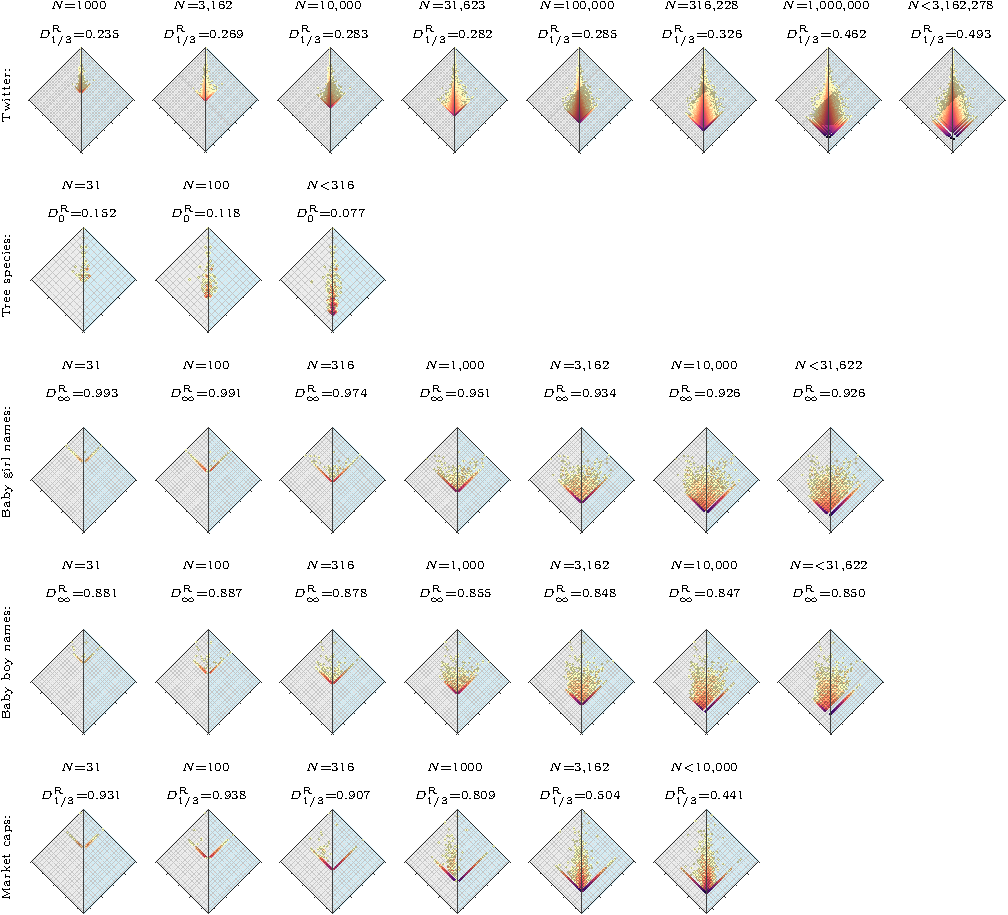
\includegraphics[width=\textwidth]{figtruncation.pdf}

We have added the following to the caption for Fig.~10:
\begin{excerpt}
  The paths of convergence towards the divergence score
  vary and may be uneven if usually monotonic,
  depending on
  the systems being compared and the choice of $\alpha$.
\end{excerpt}

We have also restructured the caption slightly to point
the reader to the flipbooks in the third sentence rather than the last.

And as the last part of our response to Reviewer 2's comment,
we have added the following to the main text at the end
of Section III F. ``Truncation Effects for Rank-Based Allotaxonographs'':
\begin{excerpt}
  We see that the values of $\rtd{\alpha}$ for the truncation
  sequences approach the `true' value in largely monotonic, if different, ways.
  The value of $\rtd{1/3}$ for the Twitter study approaches from below,
  deceptively exhibiting a flat section up to $N$=$10^{6}$.
  The ecology example starts above and moves down towards
  the overall score of $\rtd{0}$=0.077.
  Baby names and markets caps similarly both start above their
  respective overall scores for $\rtd{\infty}$ and $\rtd{1/3}$,
  and move downwards, though their scores for strong truncation
  are close to one as they appear as disjoint systems
  (their histograms are predominantly `vee'-shaped).
  While the baby name scores drop slowly and not far
  (0.993 and 0.881 for 31 names for girls and boys
  down to 0.926 and 0.850 for all names),
  the market cap study only starts to
  gain more than the `vee' shape when $N$ is into the thousands.
  Because the market cap data comparison is a blend of large-scale turnovers
  around a relatively stable core, the drop is slow and then fast and further
  (0.931 for 31 corporations down to 0.441 for all corporations).

  Our work aside, we expect any divergence measure will likely vary as orders
  of magnitude more data is included.
  And we add that in certain circumstances,
  choosing to truncate a data set may be a well justified treatment of data.

  Finally, we note that while some form of truncation is a common measurement issue with real
  data for complex systems with many components, it is certainly not the only one.
  Exploring how other kinds of measurement errors affect rank-turbulence divergence
  would be a natural area of future work.
\end{excerpt}

\begin{reviewercomment}
  Further, how does the divergence measure work in
  the presence of unbalanced list sizes, say when comparing the word
  usage of English tweets between countries?  I noticed that some
  imbalance likely appears in the baby names example.  Does the
  skewness of the underlying histogram bias the divergence and
  resulting understanding of turbulent names?
\end{reviewercomment}

We have constructed rank-turbulence divergence
(and subsequently probability-turbulence divergence)
so that they inherently accommodate uneven systems sizes.
We don't see the measure as being a bias but rather
simply capable of revealing whatever differences there
are between the systems.
With familiarity, the shape of the histogram along with the balance bars
will give the user a rich understanding of how the systems differ
(regardless of what kind of divergence is being used).

We have added two more allotaxonographs for systems of strongly different sizes
as well as an accompanying discussion.
We chose to extend the baby name section because baby names in 1880 versus 2020
provide a good example of size disparity between two systems.

As we note earlier in response to Reviewer 1,
that the first two baby name allotaxonographs are for roughly
equal populations (1968 and 2018), and that the asymmetry of the
histogram is due to the larger set of distinct names used in 2018 relative to 1968.
The relevant excerpt (from the original manuscript):

\begin{excerpt}
  We note that the asymmetries of both histograms---their apparent
  right-side `heaviness'---are not due even in part
  to changes in overall numbers.
  Using total birth numbers (see Sec. V),
  the total number of girl names recorded in 1968 and 2018
  are comparable at 1,709,551 and 1,846,101 (7.99\% increase);
  for boys, these numbers are 1,775,997 and 1,928,871 (8.61\% increase).
  The number of year-exclusive names in the 1968 and 2018
  are strikingly different however:
  8,194 and 18,029 for girls (120\% increase),
  and 4,742 and 14,004 for boys (195\% increase).
  Two of the likely major factors which have lead to this explosion in name-space
  are immigration and a cultural shift towards parents creating novel names.
\end{excerpt}

The new figures (Figs.~6 and 7) and their captions, along with the discussion excerpted follow:

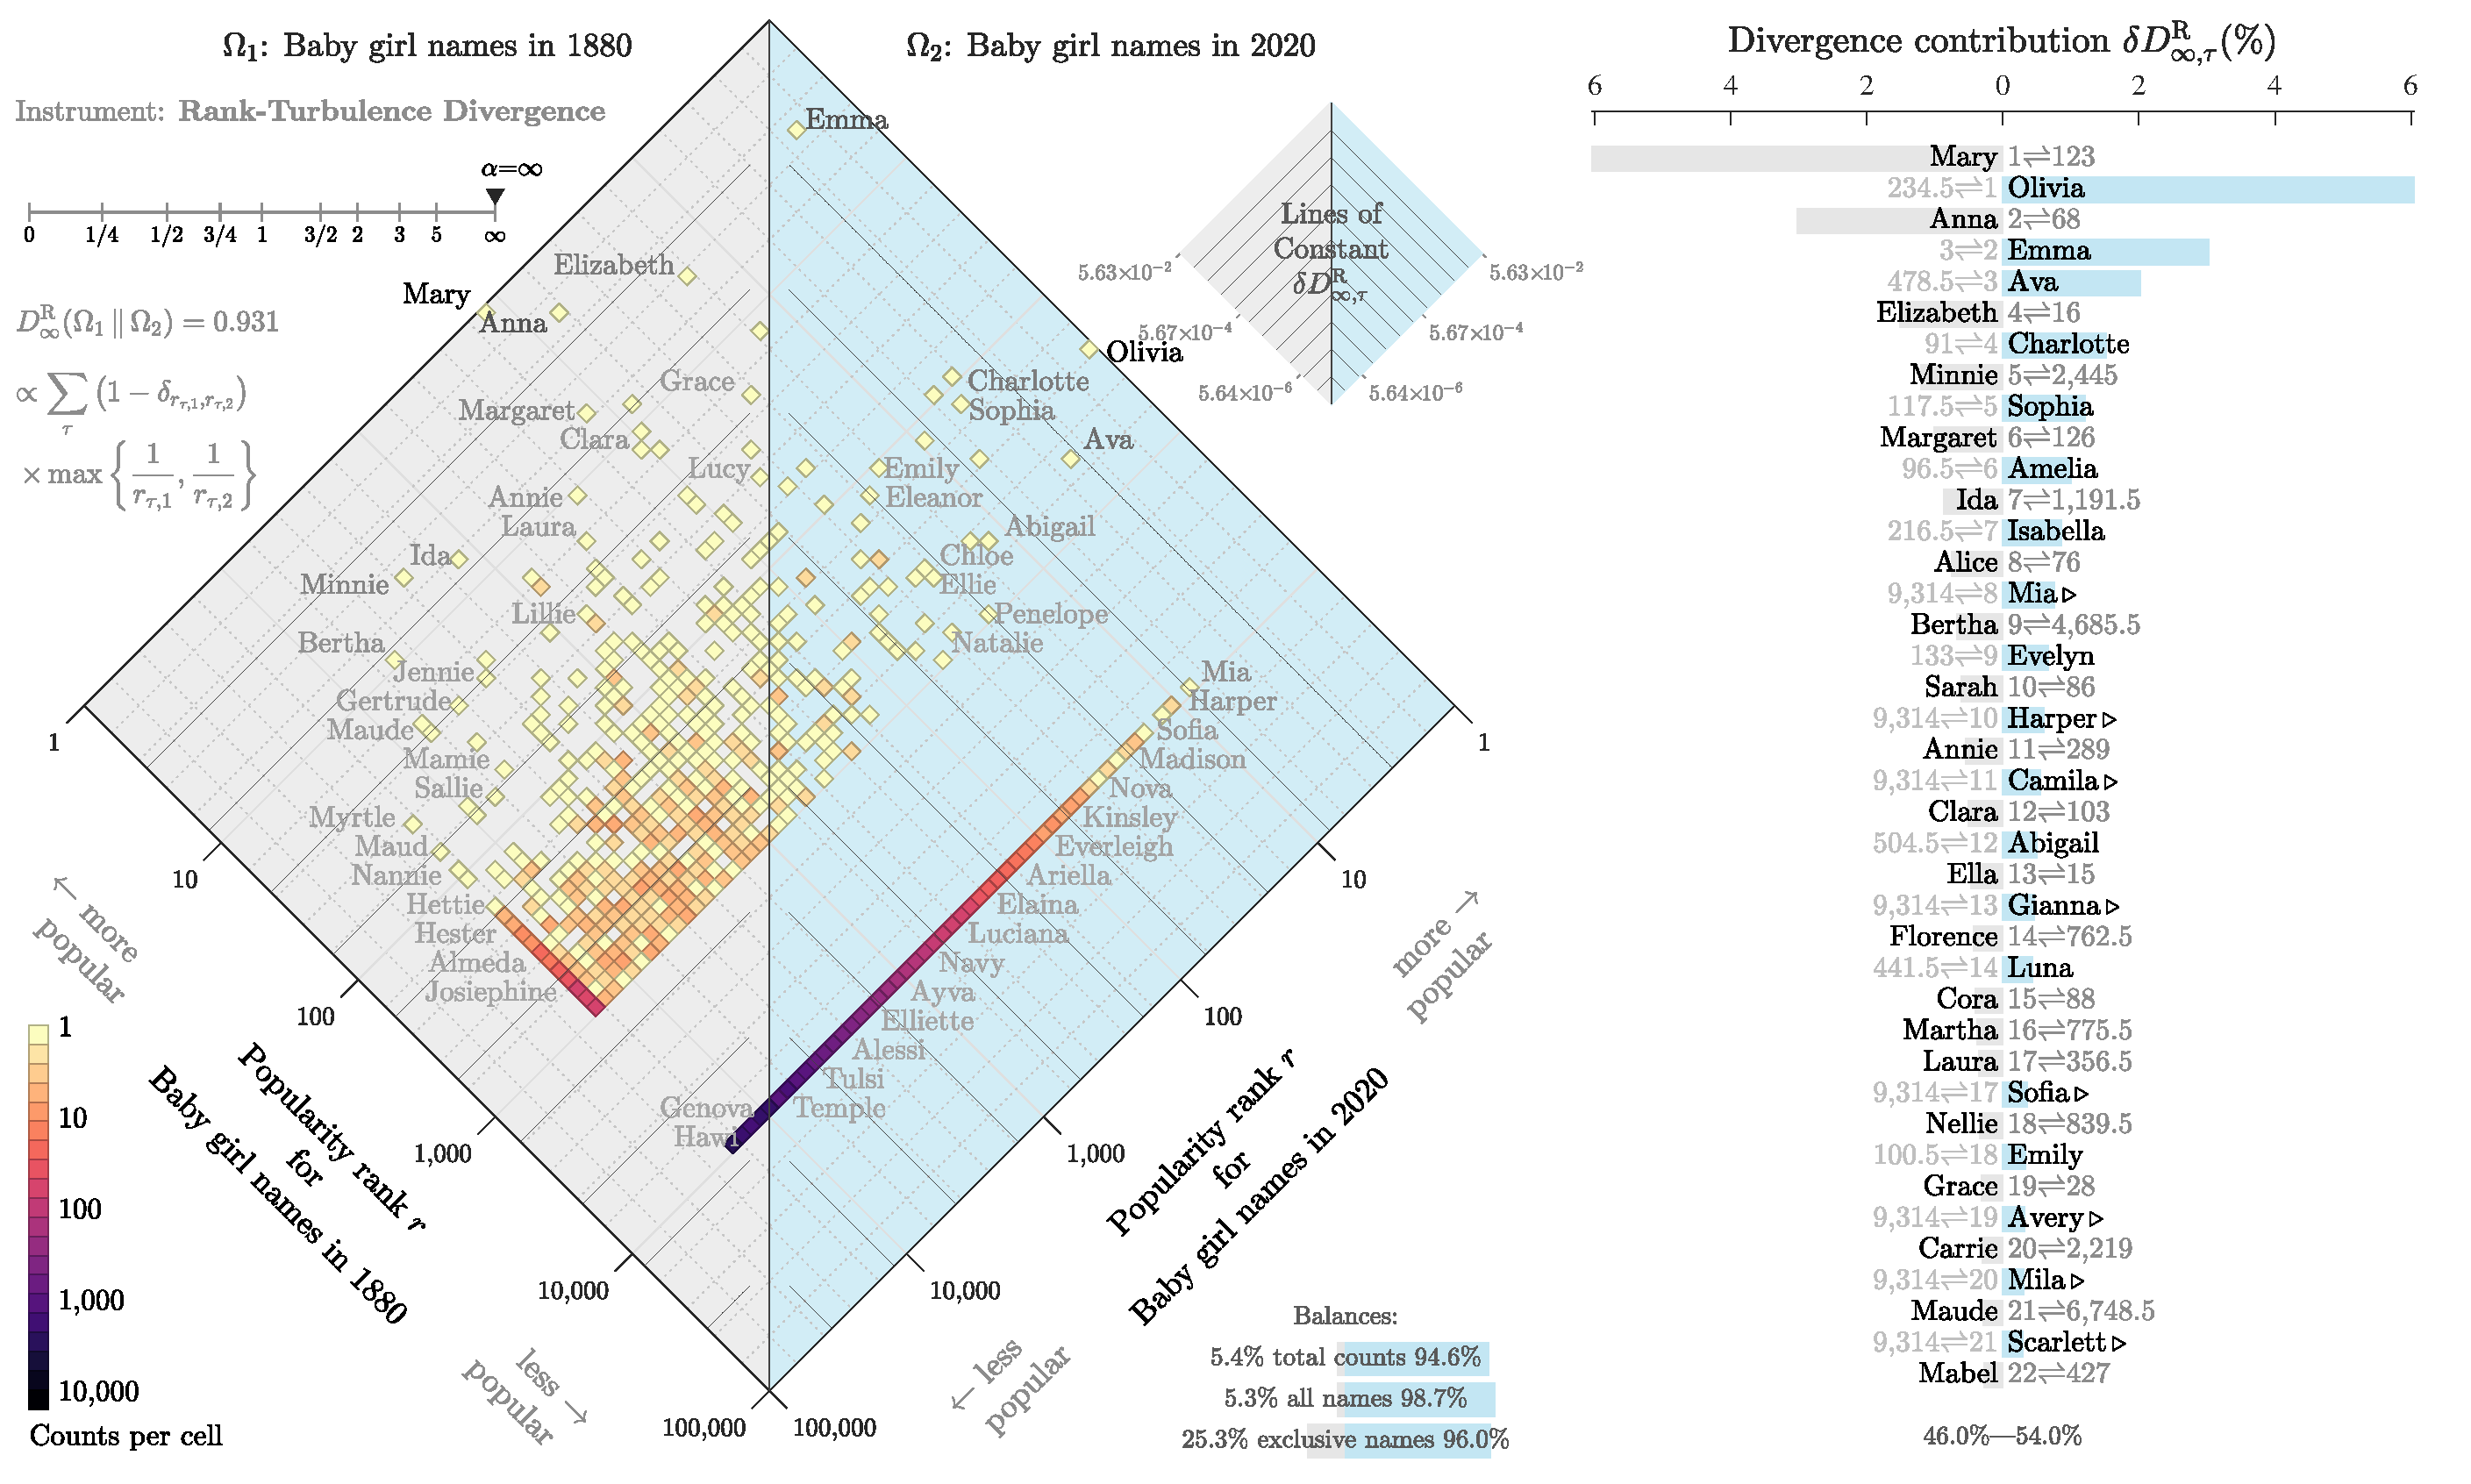
\includegraphics[width=\textwidth]{figallotaxonometer9000-babynames-rtd-010-alpha-infty-1-140-1880-vs-2020_noname.pdf}

Caption:

\begin{excerpt}
  \textbf{Allotaxonograph comparing US baby girl names for the years 1880 and 2020.}
  This figure is in part
  a demonstration of how allotaxonographs
  competently perform when the sizes of two systems differ strongly.
  For 1968 and 2018 in Fig.~5,
  the balance of total baby girl names 
  is an almost even 49.2\% and 50.8\%.
  By contrast, for 1880 and 2020, these percentages are 5.4\% versus 94.6\%.
  The choice of $\alpha=\infty$ again means that the top names for each year will
  dominate $\rtd{\infty}$, regardless of their rank in the comparison year
  (unless a name has equal rank in both years).
\end{excerpt}


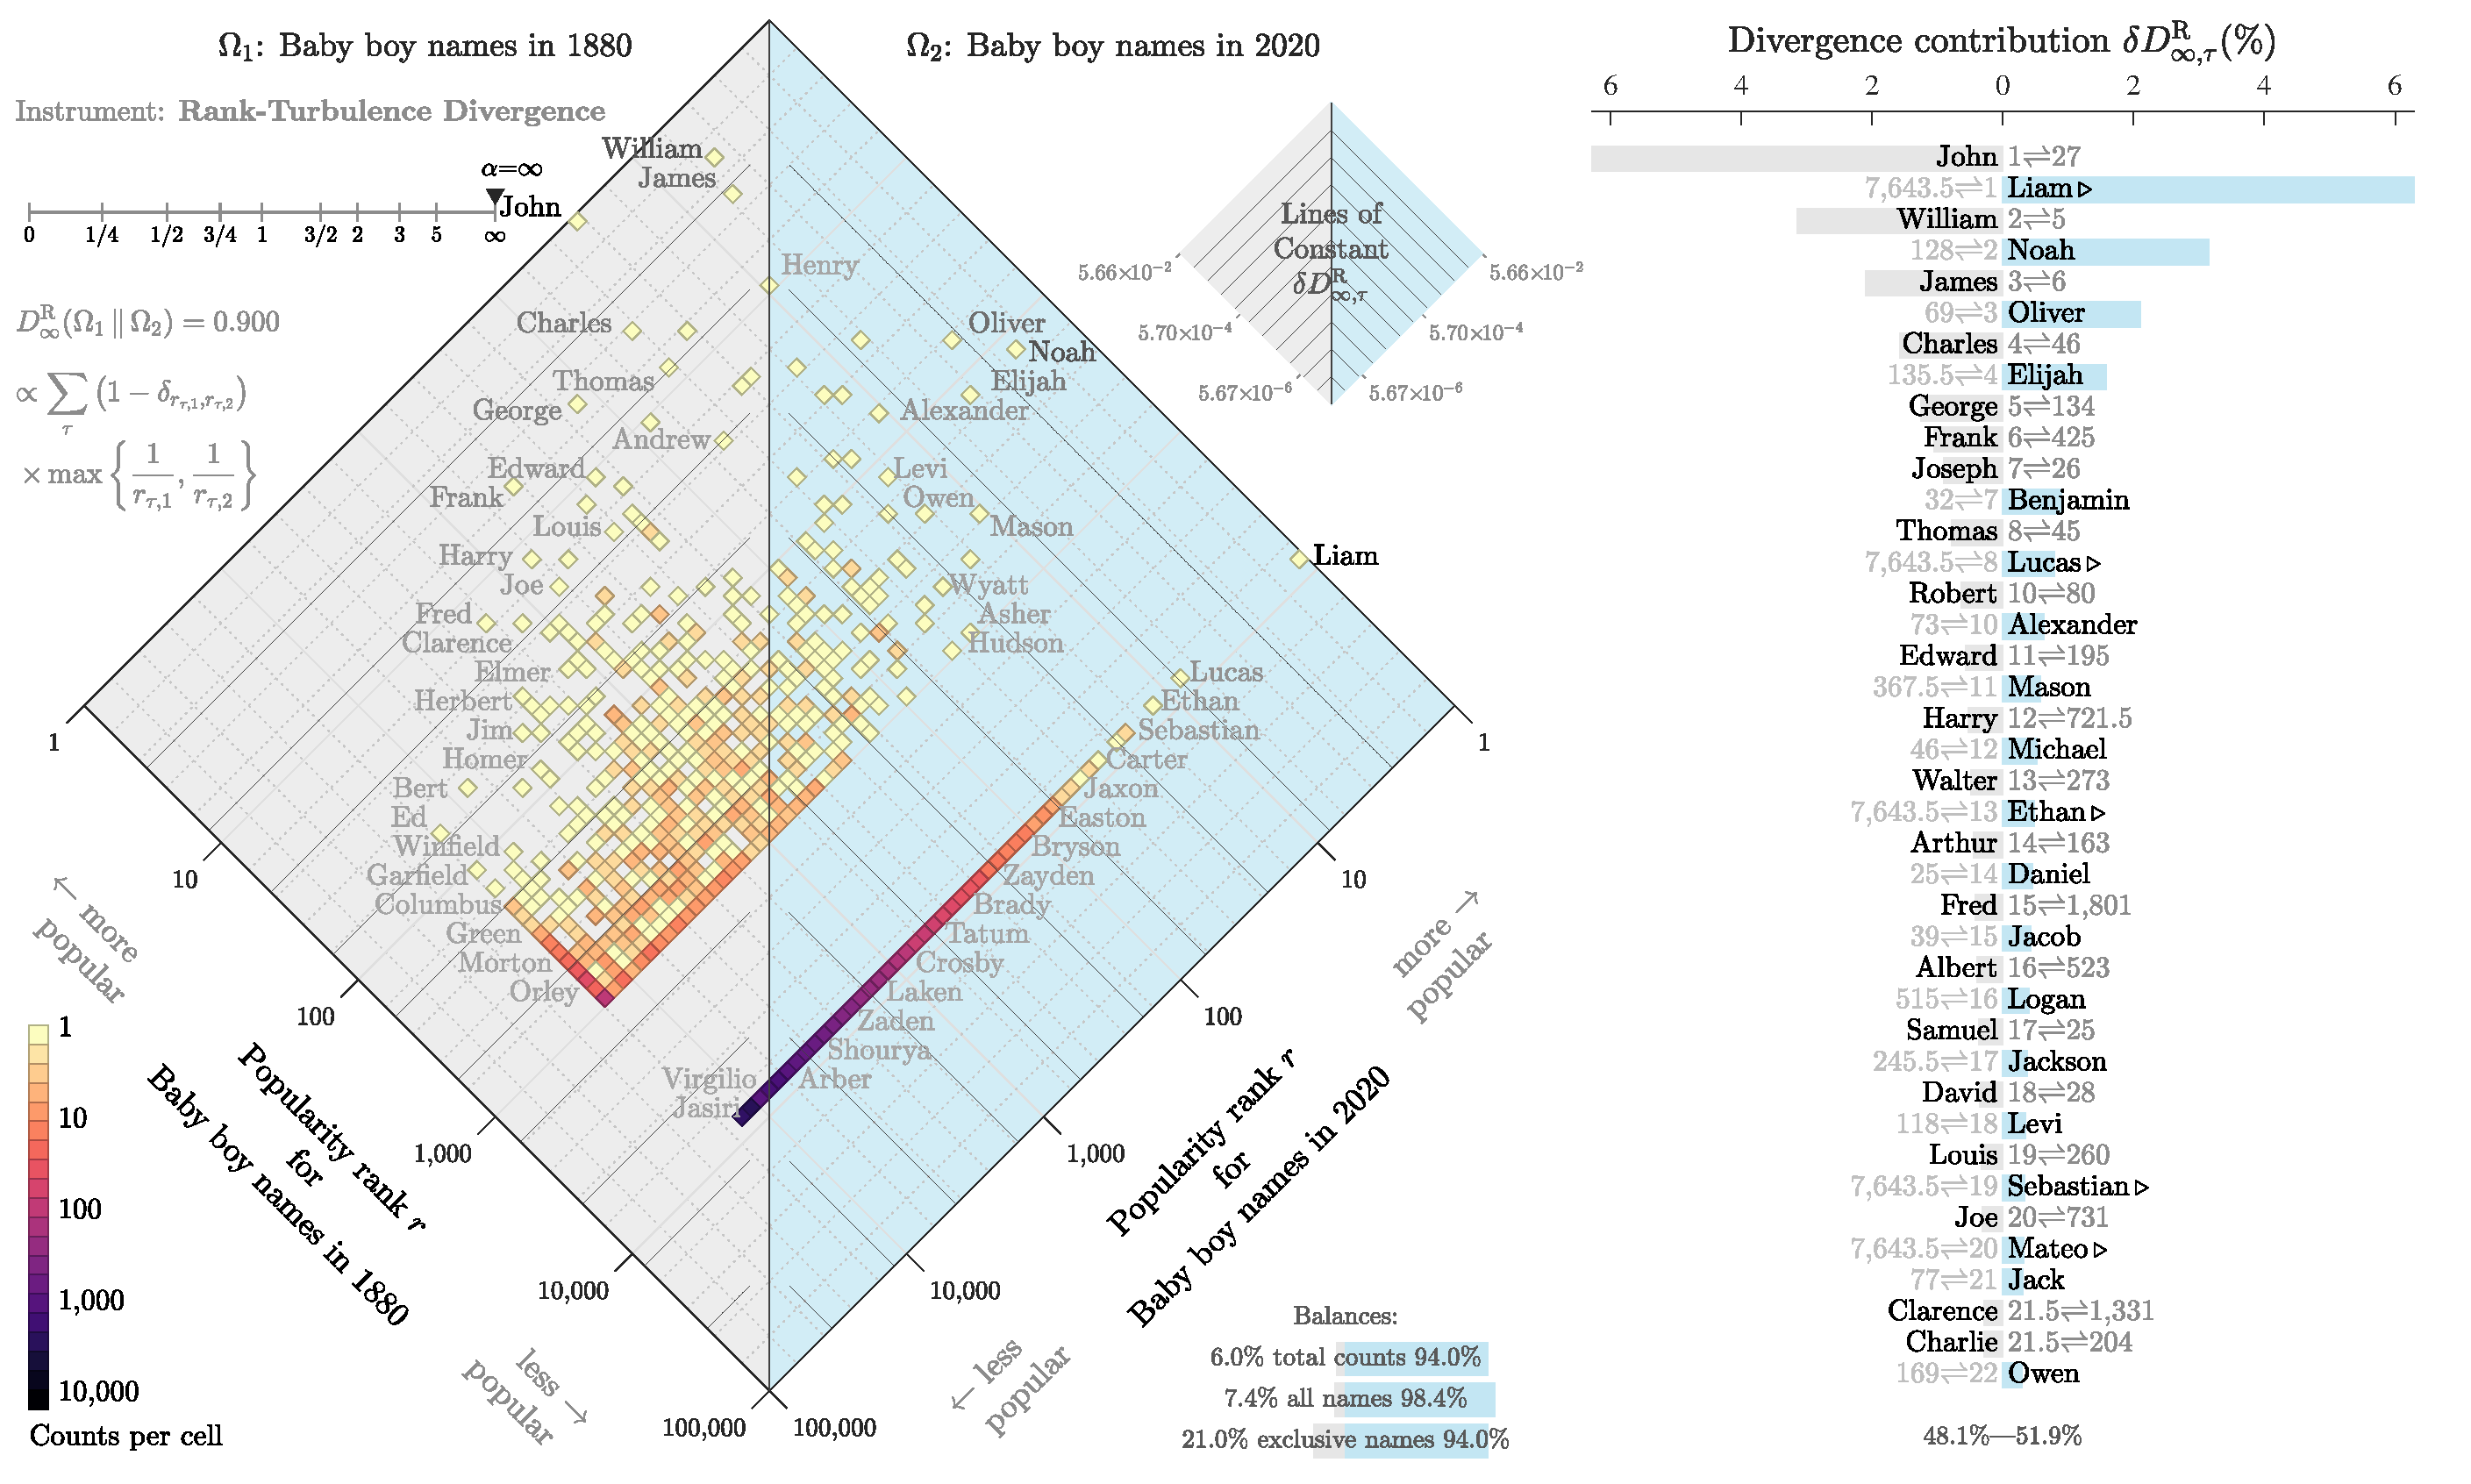
\includegraphics[width=\textwidth]{figallotaxonometer9000-babynames-rtd-010-alpha-infty-2-140-1880-vs-2020_noname.pdf}

Caption:

\begin{excerpt}
  \textbf{Allotaxonograph comparing US baby boy names for the years 1880 and 2020,
    companion to Fig~6.}
  The year 1880 has 6.0\% of the total baby boy names of both years combined,
  while 2020 has 94.0\%.
  For 1968 and 2018 in Fig.~6,
  the equivalent numbers are 49.0\% and 51.0\%.
\end{excerpt}

Added discussion.

\begin{excerpt}
  To close out our study of baby names, we add two more allotaxonographs
  whose primary purpose is to show how our instrument performs when system sizes differ strongly.
  In Figs.~6 and 7,
  we compare US baby girl and boy names in 1880 and 2020, a 140 year gap.

  We make some observations about balances,
  the rank-turbulence divergence scores,
  the rank-rank histograms,
  and
  the changes in naming from 1880 to 2020.

  For the preceding allotaxonographs
  (Figs.~1--5),
  the largest difference for system sizes has been for
  Twitter in Fig.~1.
  The date 2016/11/09 carried 59.9\% of all tweets from the two dates combined,
  with the other 41.1\% on 2017/08/18
  (top balance bar, bottom right of the histogram).

  By contrast, of the total number of baby girls born in 1880 and 2020,
  the years separately account for 5.4\% and 94.6\% respectively,
  a factor of roughly 17-fold
  (new Fig.~6)
  For boys, these weights are similar at 6.0\% and 94.0\%, around 16-fold
  (new Fig.~7).

  Because of the large increase in registered babies being born,
  the two kinds of type balances are consequently more extreme.
  For example, of the combined types for the distinct baby girl names in 1880 and 2020,
  only 5.3\% were used in 1880, while 98.7\% were used in 2020.
  For exclusive types, 25.3\% of 1880's distinct baby girl names appeared
  only in 1880, while 96.0\% of 2020's were not used in 1880.

  For baby girl names, the value of $\rtd{\infty}$=9.31 for this 140 year comparison is slightly higher
  than that for the 50 year gap between 1968 and 2018, $\rtd{\infty}$=9.26,
  while for boys the increase is from $\rtd{\infty}$=0.850 to 0.900.

  In general, the rank-rank histograms of these disparately sized systems will show a strongly separated,
  highly dense line corresponding to exclusive types on the side of the large system.
  For both baby girl and boy names in 1880 and 2020,
  the separated line is around an order of magnitude from the main body of the histogram,
  and the component cells are high count ones.
  While this separation could occur for equal-sized systems if the type counts differ enough,
  the count density of the separated line will not be as strong.
  With familiarity, a glance at the balance bars will clarify these details.

  Rank-turbulence divergence with $\alpha$=$\infty$ 
  is a function only of the highest rank for each type
  (Eq.~11).
  As such, the main contributions for girls come from
  `Mary' ($\sizerank$=1 to 123)
  `Olivia' ($\sizerank$=234.5 to 1),
  while for boys
  the leaders are
  `John' ($\sizerank$=1 to 27)
  and
  `Liam' ($\sizerank$=7,643.5 to 1, not used in 1880).

  For evolving complex systems, allotaxonographs can help lead us to 
  examine time series for individual types that occupy interesting locations
  in the rank-rank histogram.
  For baby girl names, `Emma' stands out as a name that was
  enormously popular in both
  1880 ($\sizerank$=3)
  and
  2020 ($\sizerank$=2).
  But the story for Emma proves to be akin to that of Vonnegut's man-in-a-hole's
  emotional arc [64--66].
  Ranked third in 1880, `Emma' dropped at a gradually increasing rate over the next 90 years
  to a stable set of low ranks in the 1970s---the decade of `Jennifer'---bottoming out
  at $\sizerank$=463 in 1976.
  After first starting to revive in 1983,
  `Emma' rapidly rose back to 4th in 2002 and
  stayed in the top 3 from 2003--2021,
  six times atop with $\sizerank$=1.
\end{excerpt}

\begin{reviewercomment}
  The figures function as standalone illustrations of the concepts and
  enhance the intuition underlying the measure.  I especially like
  Figure 2, which manages to compress an impressive amount of
  information into a clear visualization.

  Furthermore, the
  Supplemental Flipbooks are fantastic and I hope the publication of
  this article is accompanied by a Twitter campaign sharing these as
  gifs. I'm already excited to explore the allotaxonomy of my own
  research questions!
\end{reviewercomment}

Thank you!

As we noted in the paper, we have an online site for the papers, data, and code that we have produced
(and will produce) around allotaxonometry. There are various gifs on display!
We will make more!

The top of the code page, for example, shows a video sliding through for
season points totals for NBA players, year to year:
\url{https://compstorylab.org/allotaxonometry/code/}

Our second paper on allotaxonometry (which introduces probability-turbulence divergence)
is also available there.
While conceived as an analog of RTD,
we show that PTD has a range of very interesting properties of its own.
We also show that PTD unifies and generalizes a wide array of existing probability-based
divergences.

The main site is here:
\url{https://storylab.w3.uvm.edu/allotaxonometry/}

\reviewerheader{3}

\begin{reviewercomment}
  Reviewer \#3: This is overall an excellent piece of research. The authors develop an innovative, solid method to compare rankings in systems, and demonstrate its use for word frequencies in social media. The methods are solid, the writing of very quality and the figures as well. It is without hesitation that I recommend this paper for publication as is.
\end{reviewercomment}


We greatly, greatly appreciate Reviewer 3's extremely positive assessment. Thank you!

